\documentclass[orivec]{llncs}
\usepackage{graphicx}
\usepackage{amsmath}			% for "cases"
\usepackage{amsfonts}		% for frakur fonts
\usepackage{mathrsfs}		% for curly "E" error symbol
\usepackage{float}
\usepackage{tcolorbox}		% for wrapping example in color box
\usepackage{wrapfig}		% wrap figure beside text, used in example
\usepackage{tikz-cd}		% commutative diagrams
\usepackage{amssymb}		% for \multimap, \updownarrow, \bigstar
\usepackage{sectsty}		% change section color

% *************** Delete when not using Chinese or colors **********************
\usepackage{xeCJK}
\setCJKmainfont[BoldFont=SimHei,ItalicFont=KaiTi]{SimSun}
\usepackage{color}
\definecolor{Cerulean}{RGB}{100,100,200}
\newcommand{\emp}[1]{\textbf{\textcolor{Cerulean}{#1}}}
\definecolor{grey}{rgb}{0.9,0.9,0.9}  % grey

% \chapterfont{\color{blue}}  % sets colour of chapters
\sectionfont{\color{blue}} 
\subsectionfont{\color{blue}} 
\subsubsectionfont{\color{blue}} 

\newcommand{\vect}[1]{\boldsymbol{#1}}
\newcommand*\sigmoid{\vcenter{\hbox{
\includegraphics{sigmoid.png}}}}
\newcommand*\invsigmoid{\vcenter{\hbox{
\includegraphics{inverse-sigmoid.png}}}}
\newcommand{\invW}{\, \rotatebox[origin=c]{90}{W}}
\newcommand{\invw}{\, \rotatebox[origin=c]{90}{w}}
\newcommand*\rectifier{\vcenter{\hbox{
\includegraphics{rectifier.png}}}}
\newcommand{\dashh}{\textemdash~}

% ***** Boxed variables inside math equations
% \newcommand*{\boxedcolor}{black}
\makeatletter
% \renewcommand{\boxed}[1]{\textcolor{\boxedcolor}{%
% \fbox{\normalcolor\m@th$\displaystyle#1$}}}
% \setlength{\fboxsep}{1pt}
\renewcommand{\boxed}[1]{\fbox{\m@th$\displaystyle\scalebox{0.9}{#1}$} \,}
\makeatother

\overfullrule=0mm

\newsavebox{\MyName}
\savebox{\MyName}{
\includegraphics[scale=0.6]{YKY.png}}

\title{游荡在思考的迷宫中}
\titlerunning{游荡在思考的迷宫中}
\author{\usebox{\MyName} (King-Yin Yan)
% \\ \footnotesize{General.Intelligence@Gmail.com}
\and
Juan Carlos Kuri Pinto
}
\institute{General.Intelligence@Gmail.com}

\begin{document}

\maketitle
\setlength{\parindent}{0em}
% \setlength{\parskip}{2.8ex plus0.8ex minus0.8ex}
\setlength{\parskip}{2.8ex}


\begin{abstract}
简单介绍笔者的强人工智能理论和强化学习、动态规划、最优控制、Hamiltonian 力学系统的关系。
% 假设 $x$ 是思维状态。 在经典逻辑智能中,$x$ 是一束命题,代表当下的思考状况。 思考的过程就是不断重复进行推导: $x \vdash x' \vdash ...$。 在经典 AI 中这个作用是靠无数的逻辑 rules 来达成的。 但现在我们的做法是将 $x$ 放到向量空间中,再用一个 recurrent 神经网络来取代整个 rules base。
\end{abstract}

\section{经典逻辑 AI 背景}

Strong AI 的问题在理论上已经被\emp{数理逻辑}完整地描述了,馀下的问题是\emp{学习算法},因为在逻辑 AI 的架构下,学习算法很慢(复杂性很高),这就是我们要解决的。

我研究 logic-based AI 很多年,因此我的思路喜欢将新问题还原到逻辑 AI 那边去理解,但实际上我提倡的解决办法不是靠经典逻辑,甚至不是 symbolic 的。  但在这篇文章我还是会经常跳回到逻辑 AI 去方便理解。

用数理逻辑模拟人的思想是可行的,例如有 deduction, abduction, induction 等这些模式,详细可见《Computational logic and human thinking》by Robert Kowalski, 2011.  这些方面不影响本文的阅读。 值得一提的是,作者 Kowalski 是 logic programming,特别是 Prolog,的理论奠基人之一。

在经典逻辑 AI 中,「思考」是透过一些类似以下的步骤:
\begin{eqnarray}
\mbox{前提} & \vdash & \mbox{结论} \\
\boxed{\mbox{今天早上下雨}} & \vdash & \boxed{\mbox{草地是湿的}}
\end{eqnarray}
亦即由一些\emp{命题}(propositions)推导到另一些命题。

推导必须依靠一些逻辑的法则命题 (rule propositions),所谓「法则」是指命题里面带有 x 这样的\emp{变量}(variables):
\begin{equation}
\boxed{\mbox{地方 x 下雨}} \wedge \boxed{\mbox{x 是露天的}} \vdash \boxed{\mbox{地方 x 是湿的}}
\end{equation}
这些法则好比「逻辑引擎」的燃料,没有燃料引擎是不能推动的。

注意: 命题里面的 x,好比是有「洞」的命题,它可以透过 substitution 代入一些实物 (objects),而变成完整的命题。 这种「句子内部」(sub-propositional)的结构可以用 predicate logic (谓词逻辑)表达,但暂时不需要理会这些细节。

Logic-based AI 可以看成是将世界的「模型」压缩成一个「知识库」(knowledge-base, KB),里面装著大量逻辑式子:
\begin{equation}
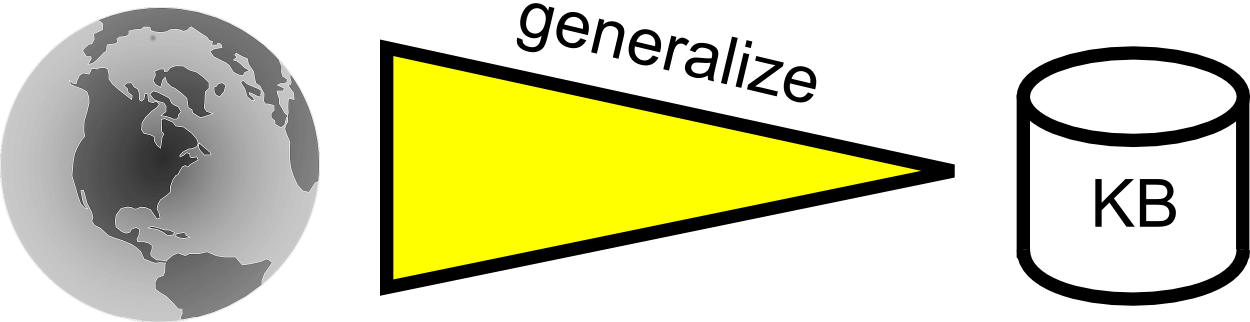
\includegraphics[scale=0.5]{world-model-compression.png}
\end{equation}
世界模型是由大量的逻辑式子经过组合而\emp{生成}的,有点像向量空间是由其「基底」生成; 但这生成过程在逻辑中特别复杂,所以符号逻辑具有很高的\emp{压缩比},但要学习一套逻辑知识库,则相应地也有极高的\emp{复杂度}。

\section{中心思想}

关键是将「思考」看成是一个\emp{动态系统} (dynamical system),它运行在\emp{思维状态} (mental states) 的空间中:
\begin{equation}
\label{fig:mental-state}
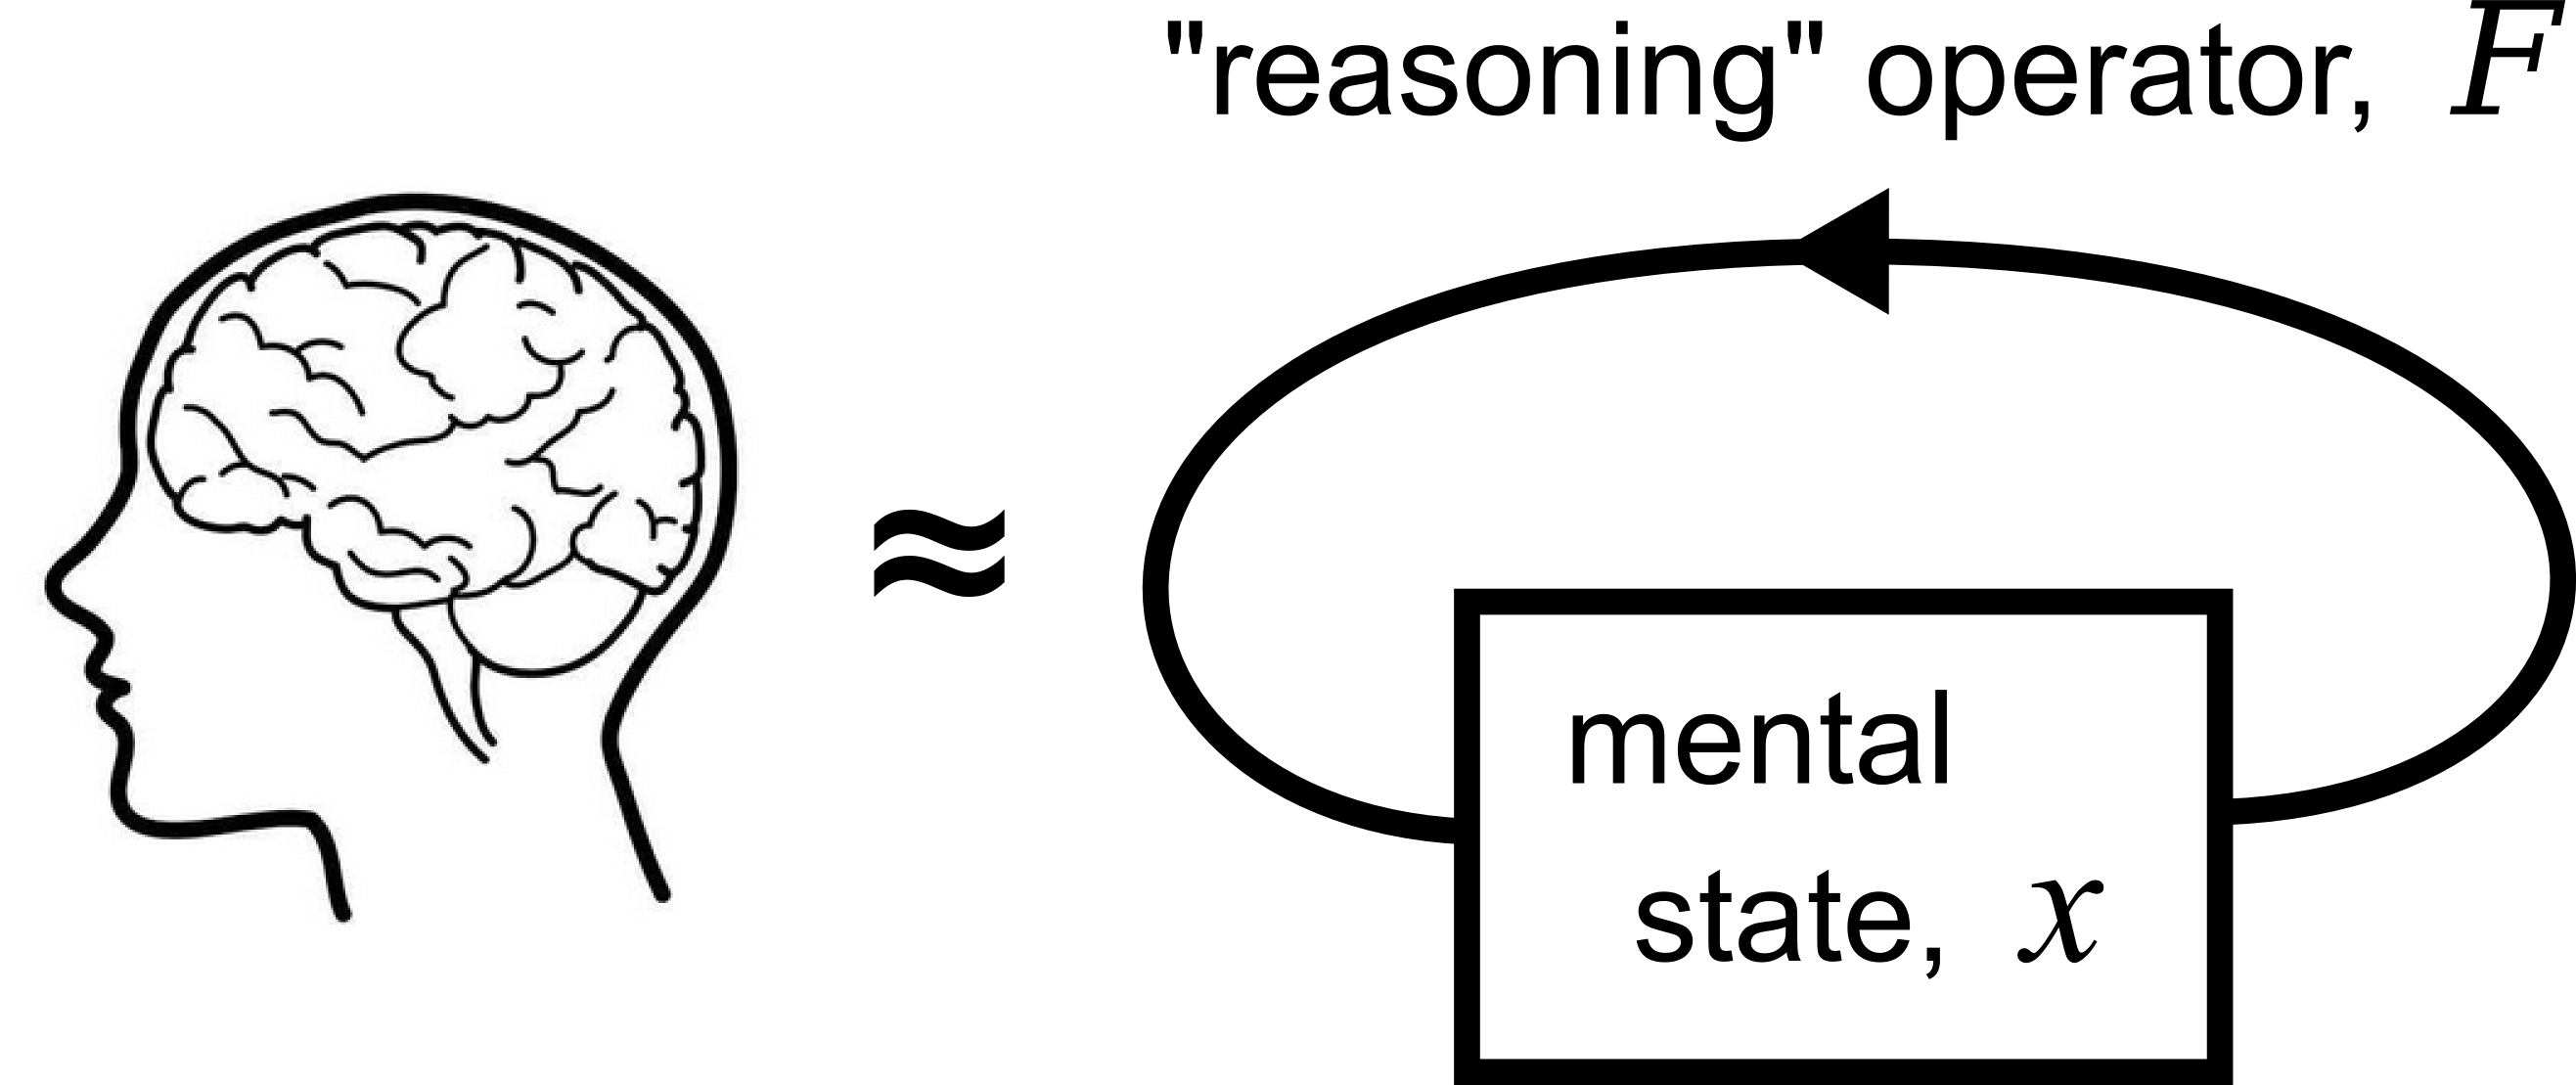
\includegraphics[scale=0.5]{mental-state.png}
\end{equation}

举例来说,一个\emp{思维状态}可以是以下的一束命题:
\begin{itemize}
\item 我在我的房间内,正在写一篇 AGI-16 的论文。
\item 我正在写一句句子的开头:「举例来说,....」
\item 我将会写一个 NP (noun phrase):「一个思维状态....」
\end{itemize}

思考的过程就是从一个思维状态 \emp{过渡} (transition) 到另一个思维状态。 就算我现在说话,我的脑子也是靠思维状态记住我说话说到句子结构的哪部分,所以我才能组织句子的语法。

思维状态是一支向量 $\vect{x} \in X$,$X$ 是全体思维空间,思考算子 (reasoning operator) $R$ 是一个 automorphism 映射: $X \rightarrow X$。

%, we would have at disposal all the tools available in vector space such as:

%\begin{itemize}
%\item numerical optimization (including gradient descent)
%\item differential equations governing time evolution
%\item dynamical systems theory, control theory (eg. adaptive filters)
%\item Lie algebra and $C^*$-algebra of continuous operators
%\item matrix theory, iteration and fixed-point theory
%\item dynamic programming (aka. reinforcement learning)
%\item neural networks and deep learning ... etc.
%\end{itemize}

换句话说: 我们将逻辑 AI 的整套器材搬到向量空间中去处理。 这个做法,部分是受到 Google 的 PageRank 和 Word2Vec \cite{Mikolov2013} 算法的启发,因为它们都是在向量空间中运作,而且非常成功。 %, both exploit the efficiency of vector and matrix calculus.

\section{控制论}

以下内容可以在一般「现代控制论」教科书中找到,例如:
\let\labelitemi\labelitemii
\begin{itemize}
\item Daniel Liberzon 2012: \textit{Calculus of variations and optimal control theory -- a concise introduction}
\item 李国勇 2008: 《最优控制理论与应用》
\item 张洪钺、王青 2005: 《最优控制理论与应用》
\end{itemize}

一个\emp{动态系统 (dynamical system)} 可以用以下方法定义:
\begin{eqnarray}
\mbox{离散时间:} \quad \quad & \vect{x}_{t+1} = \vect{F}(\vect{x}_t) \\
\mbox{连续时间:} \quad \quad & \dot{\vect{x}} = \vect{f}(\vect{x}) \label{eqn1}
\end{eqnarray}
其中 $f$ 也可以随时间改变。 如果 $f$ 不依赖时间,则系统是 time-invariant (定常的),形式上如(\ref{eqn1}) 那种微分方程叫作 autonomous (自主的)。

在我的智能系统理论里,我把 $F$ 或 $f$ 设定成 RNN (recurrent neural network),即反馈式神经网络:
\begin{eqnarray}
\mbox{离散时间:} \quad \quad & \vect{x}_{t+1} = \boxed{\mbox{RNN}}(\vect{x}_t) \\
\mbox{连续时间:} \quad \quad & \dot{\vect{x}} = \boxed{\mbox{RNN}}(\vect{x})
\end{eqnarray}
这里 recurrent 指的是它不断重复作用在 $\vect{x}$ 之上,但实际上它是一个普通的前馈式 (feed-forward) 神经网络。 注意: 在抽象理论中,$f$ 和 $F$ 可以是任意函数,我把它们设计成 NN 只是众多可能的想法之一。 之所以选用 NN,是因为它有 universal function approximator 的功能,而且是我们所知的最「聪明」的学习机器之一。

在我提出的智能系统里,$\dot{x}$ 是由\emp{學習機器}給出的,換句話說,$\dot{x}$ 是思維狀態在梯度下降至最佳狀態時的\emp{方向導數}。

一个(连续时间的)\emp{控制系统 (control system)} 定义为:
\begin{equation}
\dot{\vect{x}(t)} = f(\vect{x}(t), \vect{u}(t), t)
\end{equation}
其中 $\vect{u}(t)$ 是\emp{控制向量}。 控制论的目的就是找出最好的 $\vect{u}(t)$ 函数,令系统由初始状态 $\vect{x}_0$ 去到终点状态 $\vect{x_\bot}$。

注意: 人工智能中的 \emp{A* search},是动态规划的一个特例。 换句话说,用动态规划在某个空间中「漫游」,可以模拟到 best-first 搜寻的功能。

在这框架下,智能系统的运作可以分开成两方面: \emp{思考} 和 \emp{学习}。

\emp{思考}即是根据已学得的知识(知识储存在 RNN 里),在思维空间中找寻 $\vect{x}$ 最优的轨迹,方法是用控制论计算 $\vect{u}^*$。 $\vect{x}$ 的轨迹受 RNN 约束(系统只能依据「正确」的知识去思考),但思考时 RNN 是不变的。

\emp{学习}就是学习神经网络 RNN 的 weights $W$。 此时令 $u = 0$,即忽略控制论方面。

以上两者是两个独立的方面,但不排除它们可以在实际中同时进行。

\subsection{控制论与强化学习的关系}

在\emp{强化学习}中,我们关注两个数量:
\let\labelitemi\labelitemii
\begin{itemize}
\item $R(\vect{x},a)$ = 在状态 $\vect{x}$ 做动作 a 所获得的\emp{奖励}(reward)
\item $U(\vect{x})$ = 状态 $\vect{x}$ 的\emp{效用}(utility) 或 \emp{价值} (value) % 或 $V(\vect{x})$
\end{itemize}
简单来说,「价值」就是每个瞬时「奖励」对时间的积分:
\begin{equation}
\boxed{\mbox{价值} U} = \int \boxed{\mbox{奖励} R} \,dt
\end{equation}
(价值有时用 $V$ 表示,但为避免和势能 $V$ 混淆故不用。)

用\emp{控制论}的术语,通常定义 cost functional:
\begin{equation}
J = \int L dt + \Phi(\vect{x}_\bot)
\end{equation}
其中 $L$ 是 ``running cost'',即行走每一步的「价钱」; $\Phi$ 是 terminal cost,即到达终点 $\vect{x}_\bot$ 时,那位置的价值。

%Define a continuous version of ``utility'':
%\begin{equation}
%V(x,t) = \min_u \{ \int_t^{t_\bot} C(x,u)dt + \Phi(x_\bot,t_\bot) \} 
%\end{equation}
%where $t$ is time, $u$ is a set of control parameters, $C$ is the \emp{cost-rate} function:
%\begin{equation}
%\int C dt = R = \mbox{reward}
%\end{equation}
%This integral expresses the ``cost of the path'', whereas $\Phi(x_\bot,t_\bot)$ is the ``cost at termination''.

在\emp{分析力学}里 $L$ 又叫 Lagrangian,而 L 对时间的积分叫「作用量」:
\begin{equation}
\boxed{\mbox{作用量 (Action)}} \; S = \int L dt
\end{equation}
Hamilton 的\emp{最小作用量原理} (principle of least action) 说,在自然界的运动轨迹里,$S$ 的值总是取稳定值 (stationary value),即比起邻近的轨迹它的 $S$ 值最小。

所以有这些对应:\\
\begin{center}
\begin{tabular}{|c|c|c|}
\hline 
\emp{强化学习} & \emp{最优控制} & \emp{分析力学} \\ 
\hline
效用/价值 $U$ & 价钱 $J$ & 作用量 $S$ \\ 
\hline 
即时奖励 $R$ & running cost & Lagrangian $L$ \\ 
\hline 
action $a$ & control $u$ & (外力?) \\
\hline
\end{tabular} 
\end{center}

用比较浅显的例子: 和美女做爱能带来即时的快感 (= 奖励 $R$),但如果强奸的话会坐牢,之后很长时间很苦闷,所以这个做法的长远价值 $U$ 比其他做法较低,正常人不会选择它。

有趣的是,奖励 $R$ 对应於力学上的 Lagrangian,其物理学单位是「能量」; 换句话说,「快感」或「开心」似乎可以用「能量」的单位来量度,这和通俗心理学里常说的「正能量」不谋而合。 而,长远的价值,是以 $[\mbox{能量} \times \mbox{时间}]$ 的单位来量度。

一个智能系统,它有「智慧」的条件,就是每时每刻都不断追求「开心能量」或奖励 $R$ 的最大值,但它必需权衡轻重,有计划地找到长远的效用 $U$ 的最大值。

\subsection{经典分析力学(analytical mechanics)}

分析力学的物理内容,完全是牛顿力学的 $F = ma$,但在表述上引入了能量和 Hamiltonian 等概念,再使用微积分和变分法。

\subsubsection{Lagrange 方程}

Lagrange 引入了 Lagrangian $L = T - V$,可以分拆成\emp{動能} $T$ 和\emp{勢能} $V$ 兩部分。

重點是: \emp{動能} $T$ 是速度 $\dot{\vect{x}}$ 的函數,\emp{勢能} $V$ 是位置 $\vect{x}$ 的函數。

问题: 如果在强化学习中的「快感/奖励」对应於 Lagrangian $L$,如何在奖励之中分拆出「动能」和「势能」的分量? 

\begin{equation}
\boxed{\mbox{Lagrange equation}} \quad
\frac{d}{dt} \frac{\partial L}{\partial \dot{x}_i} - \frac{\partial L}{\partial x_i} = 0
\end{equation}
这些方程的座标是 $(\vect{x}, \dot{\vect{x}})$,可以了解成\emp{位置空间 (configuration space)}上的 tangent bundle (下述)。

\subsubsection{Hamilton 方程}

\emp{Hamiltonian} $H = T + V$,亦即总能量,但它表示成位置 $\vect{x}$ 和动量 $\vect{p}$ 的函数。

\begin{equation}
\label{Hamilton-eqns}
  \boxed{\mbox{Hamilton equation}} \quad
  \begin{cases}
      \dot{\vect{x}} & = \displaystyle \frac{\partial H}{\partial p} \\
      \dot{\vect{p}} & = - \displaystyle \frac{\partial H}{\partial x}
  \end{cases}
\end{equation}
这些方程的座标是\emp{相位空间 (phase space)} $(\vect{x}, \vect{p})$。

位置空间和相位空间之间的变换是 \emp{Legendre transformation}:
\begin{eqnarray}
\boxed{\mbox{tangent bundle}} \; T X & \rightarrow & T^* X \; \boxed{\mbox{cotangent bundle}} \\
(\vect{x}, \dot{\vect{x}}) & \mapsto & (\vect{x}, \vect{p})
\end{eqnarray}
\begin{equation}
\vect{p} = \frac{\partial L}{\partial \dot{\vect{q}}} \quad \Rightarrow \quad H := \vect{p} \dot{\vect{x}} - L
\end{equation}

\subsubsection{Hamilton-Jacobi 方程}

\begin{equation}
\boxed{\mbox{Hamilton-Jacobi equation}} \quad
H(q, \frac{\partial S}{\partial q}, t) + \frac{\partial S}{\partial t} = 0
\end{equation}
其中 $S$ 是「作用量」。 下面我们会用动态规划的原理推导出此一方程。

\subsubsection{Poisson 括号}

\begin{equation}
\label{Poisson-bracket}
\boxed{\mbox{Poisson 括号}} \quad \{ F, H \} := \sum_i \{ \frac{\partial F}{\partial q_i} \frac{\partial H}{\partial p_i} - \frac{\partial F}{\partial p_i} \frac{\partial H}{\partial q_i} \}
\end{equation}
在力学系统中,它表示任意一力学量(函数 $f$)对时间的改变量:
\begin{equation}
\dot{f} = \{ f, H \} 
\end{equation}
\begin{equation}
\frac{\partial}{\partial t} = \frac{\partial}{\partial p} \dot{p} + \frac{\partial}{\partial q} \dot{q}
\end{equation}
以上使用了微分的 chain rule,但由於 $\dot{\vect{p}}$ 和 $\dot{\vect{q}}$ 可以由 Hamilton 方程 (\ref{Hamilton-eqns}) 给出,所以得到 Poisson 括号的形式 (\ref{Poisson-bracket})。

每个物理学生都知道的「经典-量子对应原理」:
\begin{equation}
[\vect{F}, \vect{G}] \quad \Leftrightarrow \quad i \hbar \{ F, G \}
\end{equation}
这对应原理是 P.A.M. Dirac 发现的。

在经典力学里,
\begin{equation}
\{ \vect{x}, \vect{p} \} = 1
\end{equation}
但在量子力学里,
\begin{equation}
[ \vect{X}, \vect{P} ] = i \hbar
\end{equation}
这也是 Heisenberg 测不准原理的由来:
\begin{equation}
\Delta \vect{X} \Delta \vect{P} \ge \frac{\hbar}{2}
\end{equation}

如果在某一流形上,「广义」Poisson 括号是 nondegenerate (非退化)的,则它变成了\emp{辛流形}结构的 $\omega = \{ \cdot, \cdot \}$ 括号 (下述)。

\subsection{Hamiltonian 的出现}

考虑一个典型的控制论问题,系统是:
\begin{eqnarray}
\mbox{状态方程:} \quad & \dot{\vect{x}}(t) = \vect{f}[\vect{x}(t), \vect{u}(t), t] \\
\mbox{边值条件:} \quad & \vect{x}(t_0) = \vect{x}_0 \,,\, \vect{x}(t_\bot) = \vect{x}_\bot \\
\mbox{目標函数:} \quad & J = \int_{t_0}^{t_\bot} L[\vect{x}(t), \vect{u}(t), t] dt
\end{eqnarray}
要找的是最优控制 $\vect{u}^*(t)$。

\begin{figure}[H]
\begin{center}
\colorbox{grey}{\parbox{0.95\textwidth}{\setlength{\parskip}{2.5ex}

\emp{Lagrange multiplier} 是找极大/小值的常用方法: 如果我们要找:
\begin{equation}
\max \; f(x) \quad \mbox{ subject to } \quad g(x) = 0
\end{equation}
Lagrange 建议我们建构 Lagrangian 函数:
\begin{equation}
L(x, \lambda) = f(x) - \lambda g(x)
\end{equation}
然后求解:
\begin{equation}
\nabla_{x,\lambda} L = 0
\end{equation}
}}
\end{center}
\end{figure}

现在将 Lagrange multiplier 方法应用到我们的问题上,会发现新的目标函数是:
\begin{equation}
J = \int_{t_0}^{t_\bot} \{ L + \vect{\lambda}^T(t) \left[ f(\vect{x}, \vect{u}, t) - \dot{\vect{x}} \right] \} dt
\end{equation}
因此可以引入一个新的标量函数 $H$,即 Hamiltonian:
\begin{equation}
H(\vect{x}, \vect{u}, t) = L(\vect{x}, \vect{u}, t) + \vect{\lambda}^T(t) f(\vect{x}, \vect{u}, t)
\end{equation}
物理学上,$\vect{f}$ 的单位是速度,而 $L$ 的单位是能量,所以 $\lambda$ 应该具有 \emp{动量} 的单位。

\subsubsection{极小值原理}

Lev Pontryagin (1908-1988) 提出了 \emp{极小值原理},是经典变分法的推广。 经典变分法的最优条件是:
\begin{equation}
\frac{\partial H}{\partial \vect{u}} = \vect{0}
\end{equation}
极小值原理将最优条件改成是:
\begin{equation}
\min_{u \in \Omega} H(\vect{x}^*, \vect{\lambda}^*, \vect{u}, t) = H(\vect{x}^*, \vect{\lambda}^*, \vect{u}^*, t)
\end{equation}
即是说: 在最优轨迹 $\vect{x}^*(t)$ 和最优控制 $\vect{u}^*(t)$ 上,$H$ 取最小值。 它的好处是,当 $\displaystyle \frac{\partial H}{\partial \vect{u}}$ 不连续或不存在时,或者 $\vect{u}$ 受其他约束时,也可以应用。

粗略来说,极小值原理比经典变分法更一般,而动态学习又比极小值原理更一般。

\subsubsection{Hamilton-Jacobi-Bellman 方程}

\begin{itemize}
\item Stanislaw Zak (2003): \textit{Systems and control}
\end{itemize}

% \S 5.4.3 Zak.

用动态规划的 \emp{Bellman optimality condition} 可以推导出微分形式的 Hamilton-Jacobi-Bellman 方程。  重温一下,Bellman 最优条件说的是: 「从最优路径末端切去一小截之后,馀下的还是最优路径。」  它通常写成如下的 recursive 形式:
\begin{eqnarray}
\boxed{\mbox{最优路径}} & = & \mbox{在小段上选取最大奖励} + \boxed{\mbox{馀下的最优路径}} \\
J^*_t & = & \max_{u} \{ \boxed{\mbox{奖励}(u, t)} + J^*_{t-1} \}
\end{eqnarray}

\begin{equation}
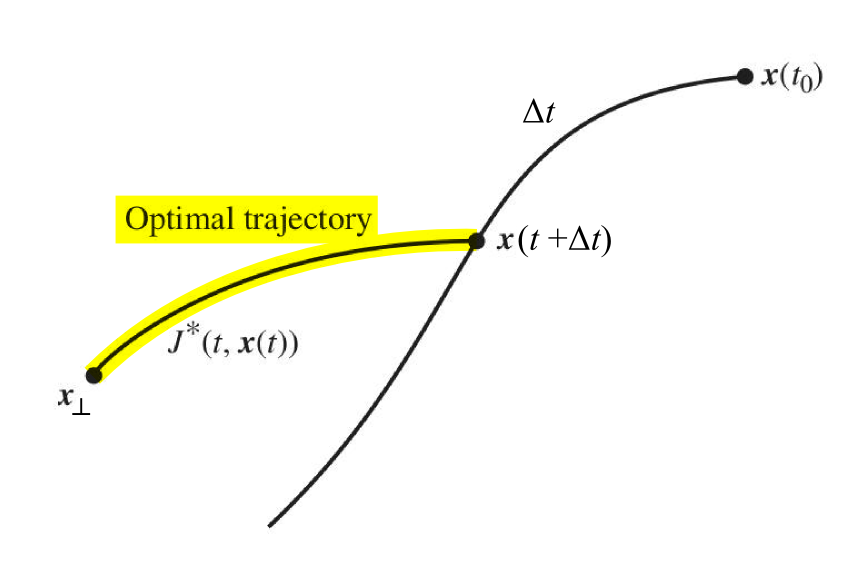
\includegraphics[scale=0.4]{optimal-trajectory.png}
\end{equation}

我们在时间 interval 的开端切出一小段:
\begin{equation}
[ t_0, t_\bot ] = [ t_0, t_0 + \Delta t ] \cup [ t_0 + \Delta t, t_\bot ]
\end{equation}
我们想优化的目标函数是:
\begin{equation}
J^*(t, \vect{x}, \vect{u}) = \min_u \{ \int_{t_0}^{t + \Delta t} L d\tau + \int_{t + \Delta t}^{t_\bot} L d\tau + \Phi(t_\bot, \vect{x}_\bot) \}
\end{equation}
根据 Bellman 条件,目标函数变成:
\begin{equation}
J^*(t, \vect{x}) = \min_u \{ \int_{t_0}^{t + \Delta t} L d\tau + J^*(t + \Delta t, \vect{x}(t + \Delta t)) \}
\end{equation}
用 Taylor series 展开右面的 $J^*$:
\begin{equation}
J^* + \frac{\partial J^*}{\partial t} \Delta t + \frac{\partial J^*}{\partial \vect{x}}(\vect{x}(t + \Delta t) - \vect{x}(t)) + \mbox{H.O.T.}
\end{equation}
左右两边的 $J^*$ 互相消去,而且 $\vect{x}(t + \Delta t) - \vect{x}(t) \approx \dot{\vect{x}} \Delta t$,於是有:
\begin{equation}
0 = \min_u \{ \int_{t_0}^{t + \Delta t} L d\tau + \frac{\partial J^*}{\partial t} \Delta t + \frac{\partial J^*}{\partial \vect{x}} \dot{\vect{x}} \Delta t + \mbox{H.O.T.} \}
\end{equation}
又由於 $\Delta t$ 很小,而且 $\dot{\vect{x}} = \vect{f}$,所以:
\begin{equation}
0 = \min_u \{ L \Delta t + \frac{\partial J^*}{\partial t} \Delta t + \frac{\partial J^*}{\partial \vect{x}} \vect{f} \Delta t + \mbox{H.O.T.} \}
\end{equation}
全式除以 $\Delta t$ 并令 $\Delta t \rightarrow 0$:
\begin{equation}
0 = \frac{\partial J^*}{\partial t} + \min_u \{ L + \frac{\partial J^*}{\partial \vect{x}} \vect{f} \}
\end{equation}
记得 Hamiltonian 的定义是 $\displaystyle H = L + \frac{\partial J^*}{\partial \vect{x}} \vect{f}$,所以得到想要的结果:
\begin{equation}
\boxed{\mbox{Hamilton-Jacobi equation}} \quad
0 = \frac{\partial J^*}{\partial t} + \min_u H
\end{equation}

% The differential version is the Hamilton-Jacobi equation:
% \begin{equation}
% \frac{d}{dt} V(x,t) = \min_u \{ C(x,u) + \langle \nabla V(x,t), f(x,u) \rangle \} 
% \end{equation}
% where $x$ must obey this dynamics:
% \begin{equation}
% \dot{x}(t) = f(x(t),u(t)).
% \end{equation}

这个方程和量子力学中的 \emp{Schr\"{o}dinger equation} 很相似:
\begin{equation}
i \hbar \frac{\partial}{\partial t} \Psi(x,t) = \left[ V(x,t) + \frac{-\hbar^2}{2\mu} \nabla^2 \right] \Psi(x,t).
\end{equation}
其中 $\Psi$ 类似於我们的 $J$ (或许 $\Psi$ 是自然界希望取极值的某种东西?)

\subsection{Symplectic 结构}

\begin{itemize}
\item Stephanie Singer (2001): \textit{Symmetry in mechanics -- a gentle, modern introduction}
\item 锺万勰 2011: 《力、功、能量与辛数学》
\end{itemize}

Symplectic 的拉丁文意思是「互相交错 (intertwined)」,它用来描述 Hamiltonian 系统的几何结构。 中文译作「辛」是音译。  Symplectic 概念是 Hermann Weyl 研究 Hamilton 系统的对称性时在 1939 年提出的。

在数值计算上,处理 Hamilton 系统时,如果算法尊重 symplectic 结构(叫 symplectic integrators),会比一般的算法更准确; 而一般解微分方程的算法,例如 Euler 算法和 Runge-Kutta 算法,有时会给出错误的结果。

举例来说,从 Hamiltonian 的角度来看,动量 $p$ (momentum) 和 速度 $v$ (velocity) 是成\emp{对偶}的,$p$ 总是伴随 $v$ 出现,因为 $p \cdot v = mv^2$ 的单位是能量。

举另一个例子,假设我们有两个用来定义系统状态的向量:
\begin{equation}
x_1 = \left(
\begin{array}{c}
s_1\\
f_1\\
\end{array}
\right), \quad
x_2 = \left(
\begin{array}{c}
s_2\\
f_2\\
\end{array}
\right)
\end{equation}
其中 $s$ 是位移(单位是长度),$f$ 是力。 这两个向量的「辛内积」定义为:
\begin{eqnarray}
\langle x_1, x_2 \rangle & = & x_1^T \, J \, x_2 \nonumber \\
& = &
\left(
\begin{array}{c}
s_1\\
f_1\\
\end{array}
\right)^T
\left( \begin{array}{cc}
0  & I \\
-I & 0 \end{array} \right)
\left(
\begin{array}{c}
s_2\\
f_2\\
\end{array}
\right) \\
& = & f_2 s_1 - f_1 s_2 \nonumber
\end{eqnarray}
其中矩阵 $J$ 就是辛的微分形式 $\omega$ 的结构矩阵(下述)。 由於 $f \cdot s$ 表示的是「所做的功」,上式表示的是
\begin{multline}
(\mbox{状态1的力对状态2的位移所做的功}) - \\
(\mbox{状态2的力对状态1的位移所做的功})
\end{multline}
也就是「相互功」,辛正交则 $\langle x_1, x_2 \rangle = 0$,代表 work reciprocity(功的互等),所以辛几何是一种关於能量的代数。

在微分几何里,研究抽象的 Hamiltonian systems,会发现 symplectic 结构。 这结构用微分流形 $M$ 及其上的一个 微分形式 (differential form) $\omega$ 来定义。 需要一些微分几何的基础.....

\subsubsection{Vectors and co-vectors}

Vector 和 co-vector 之间的关系,可以看成是「$d$ 别人的东西」和「被别人 $d$ 的东西」,这里 $d$ 表示微分。

「$d$ 别人的东西」是线性的 differential operators,记作 $\displaystyle \frac{\partial}{\partial x_1}$、$\displaystyle \frac{\partial}{\partial x_2}$ 等;它们很自然地组成一个 vector space $T_x M$。

「被别人 $d$ 的东西」是一些线性的微分形式,记作 $dx_1$、$dx_2$ 等; 它们属於 $T_x M$ 的 dual space。

\subsubsection{Manifolds}

基本上「流形」的意思是「弯曲的空间」,它们局部地近似於 Euclidean 空间 $\mathbb{R}^n$,局部的座标可以分段用一组微分映射来描述,这些 maps 叫 charts。
\begin{equation}
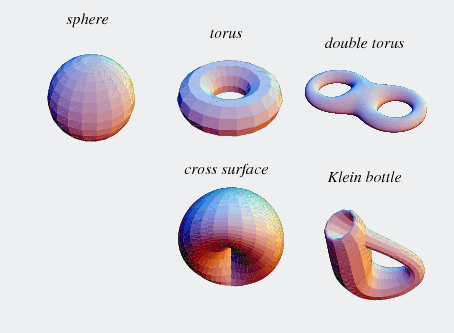
\includegraphics[scale=0.5]{smooth-manifolds.png}
\end{equation}

\subsubsection{Phase space}

「相位空间」指的是力学系统里,$i$ 个粒子的位置 $x_i$ 和动量 $p_i$ 合并而成的 $(\vect{x}, \vect{p})$ 空间。 但 configuration space 指的是所有可容许的位置 $\vect{x}$ 的空间。

\subsubsection{Vector fields, differential forms, Hamiltonian flow}

根据 Hamilton 方程,再用微分的 chain rule 可以得到:
\begin{equation}
\frac{d}{dt} = \frac{\partial H}{\partial \vect{p}} \frac{\partial}{\partial \vect{x}} - \frac{\partial H}{\partial \vect{x}} \frac{\partial}{\partial \vect{p}}
\end{equation}
它是一个微分算子,亦即是\emp{向量场}; 它有个特别的名字叫 Hamiltonian flow $\vec{H}$ (很多书记作 $X_H$):
\begin{equation}
\vec{H} := \frac{d}{dt} = \{ \cdot, H \}
\end{equation}
可以看出 $\vec{H} H = \{ H, H \} = \frac{dH}{dt} = 0$ 就是\emp{能量守恒}的形式。

Hamilton 系统的动态方程就是:
\begin{equation}
\dot{\vect{x}} = \vec{H}
\end{equation}
所以在我们的智能系统中,RNN 可以看成是 $\vec{H}$。

\begin{eqnarray}
\omega & = & \sum_i dx_i \wedge dp_i \\
\omega(\vec{H}, \cdot) & = & dH
\end{eqnarray}
我暂时不很明白它的意义。

我们说 Hamiltonian flow 保持 (preserve) 辛结构。 假设 $\Gamma_t(\vect{x}_0) = \vect{x}(t)$ 描述 Hamiltonian flow 的轨迹; $\Gamma_0(\vect{x}) \equiv \vect{x}$。 The \emp{pullback} of $\omega$ along $\Gamma$ is still $\omega$:
\begin{equation}
\Gamma^*_t \omega = \omega
\end{equation}
\begin{equation}
\vec{H} H = 0 \quad \mbox{is equivalent to} \quad \Gamma^*_t \omega = \omega
\end{equation}

\subsubsection{Tangent and co-tangent bundle}

在流形上每点有一个 tangent space,所谓 tangent bundle 是指流形上每点 $x$ 的 tangent space $T_x M$ 的总和:
\begin{equation}
TM := \bigcup_{x \in M} T_x M
\end{equation}
\begin{equation}
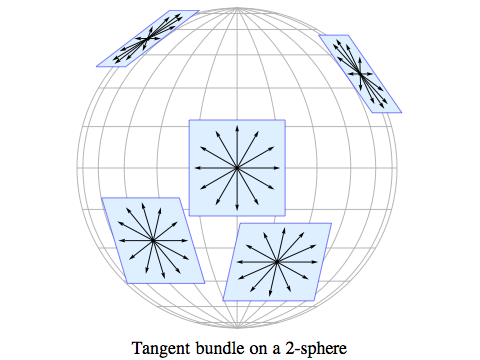
\includegraphics[scale=0.5]{tangent-bundle.png}
\end{equation}
\begin{equation}
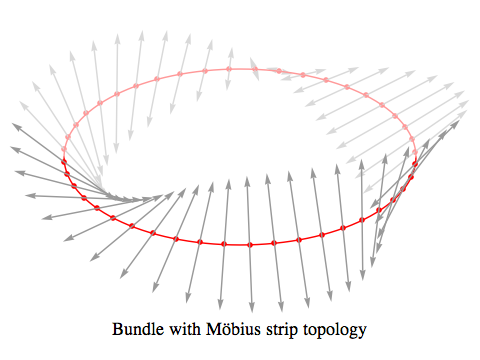
\includegraphics[scale=0.5]{tangent-bundle-2.png}
\end{equation}

粗略地,tangent bundle 可以看成是 $M \times T_x M$,而 $M$ 和 $T_x M$ 的维数都是 $n$,所以 tangent bundle 的维数是 $2n$。 在力学上,\emp{cotangent bundle} 就是相位空间 $(\vect{x}. \vect{p})$ 的空间 (The phase space of a mechanical system is the cotangent bundle of its configuration space)。

\subsubsection{Push forward, pull back}

\subsubsection{Energy conservation, area form}

(Stephanie \S 4.4)

\subsubsection{Symmetry of Hamiltonian system, Lie groups}

Symplectic groups 是一些保存辛结构的变换 $T$ 的群:
\begin{equation}
\omega(T x, T y) = \omega(x, y) \quad \forall x, y \in V
\end{equation}
$V$ 是向量空间。 在 $V$ 上的 symplectic 变换的全体记作 $Sp(V)$。

\subsubsection{Momentum maps}

\subsection{动态系统理论}

\subsubsection{Floer homology}

\emp{Homology (同调论)} 研究的是空间中「有没有穿洞」的樸拓结构。 最简单的 \emp{singular homology} 是将空间用三角形剖分 (triangulation),然后透过著名的 Euler formula $V + F = E + 2$ 及其扩充,让我们可以计算 Euler characteristic $\chi$,此即空间穿洞的个数。
\begin{equation}
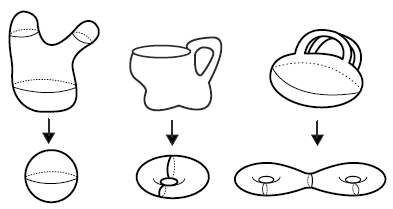
\includegraphics[scale=0.5]{manifolds-with-holes.png}
\end{equation}

\begin{equation}
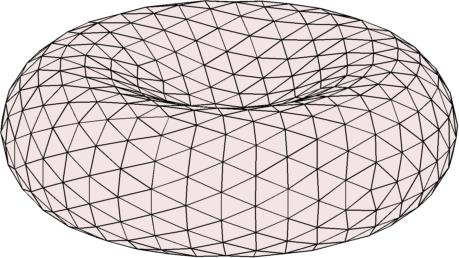
\includegraphics[scale=0.25]{torus-triangulation.jpg}
\end{equation}
当这些三角形剖分趋於无穷小时,我们得到用微分形式 (differential forms) 描述的 homology,即 \emp{de Rham homology}。 

\begin{equation}

\includegraphics[scale=0.5]{height-function.png}
\end{equation}
在流形上定义一个 potential function,例如简单的 height function,就可以做 Morse theory,这时每个点可以根据势能函数向下流 (gradient flow),流到一些最低位置,它们是临界点 (critical points)。 Morse decomposition 将空间用这些临界点分割(流到同一临界点的 flows 认作同一 equivalent class),得到的是 \emp{Morse homology}。
\begin{equation}
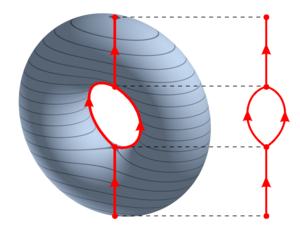
\includegraphics[scale=0.5]{gradient-flow.png}
\end{equation}

\emp{Floer homology} 是 Morse homology 的\textbf{无限维空间}版本,比较难计算。

\subsubsection{Conley theory}

\subsubsection{Entropy, ergodicity}

\subsubsection{Lie algebra 的另一应用}

例如一架车可以有两个基本动作: (A) 绕中心旋转、或 (B) 前后行驶,它们的 Lie 括号 $[A,B]$,产生出的动作是左右方向行驶,这类似於「平行泊车」的时候,车子的移动方向:
\begin{equation}
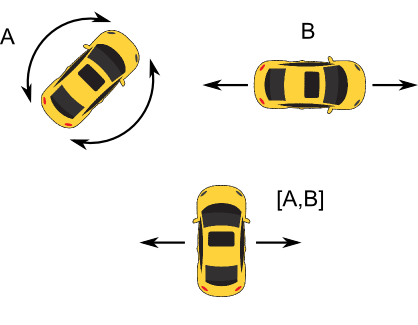
\includegraphics[scale=0.5]{Lie-bracket-car.png}
\end{equation}

(可控性与 ``reachable'' 概念。)

\subsubsection{Stable, unstable, and center manifold}

\subsubsection{Smale horseshoe}

\section{最优控制的计算方法}

\subsubsection{直接法}

\subsubsection{间接法}

\subsubsection{Lyapunov 函数第一方法}

\subsubsection{Lyapunov 函数第二方法}

\clearpage
\section{Jacobian 神经网络学习算法}

经典的神经网络 Back Prop 学习算法,它是一个 error-driven 算法,但在很多人工智能的实际应用中,不存在唯一的「理想答案」,而是根据正或负的奖励 (reward) 学习。  当答案正确时,奖励 $> 0, \mbox{error} = 0$; 当答案不正确时,奖励 $< 0$,但 $\mbox{error}$ 仍是不知道的(因为不知道理想答案)。  简言之,就是不能用 error-driven 学习。 

所以我想出了一个 reward-driven 的学习法: 假设神经网络将 $\vect{x}_0 \mapsto \vect{y}_0$,它通常也会将 $\vect{x}_0$ 的邻域 map 到 $\vect{y}_0$ 的邻域。 如果我们想「加强」这个映射,可以将「更大的 $\vect{x}_0$ 的邻域」映射到「接近 $\vect{y}_0$ 的邻域」。

这种算法对人工智能应该很重要,暂时我还想不出有什么其他办法,可以做到[深度]神经网络的 reward-driven 学习。 

将这思想更准确化,可以将 feed-forward 神经网络的构造看成是这样的:
\begin{eqnarray}
\vect{y} &=& \vect{F}(\vect{x}) \\
\vect{y} &=& \sigmoid \stackrel{_L}{W} ... \sigmoid \stackrel{_\ell}{W} ... \sigmoid \stackrel{_1}{W} \vect{x}
\end{eqnarray}
其中 $W$ 代表每一层 (layer) $\ell$ 的矩阵。

$F$ 的\textbf{反方向}是:
\begin{eqnarray}
\vect{x} &=& \vect{F}^{-1}(\vect{y}) \\
\vect{x} &=& \stackrel{_1}{\invW} \invsigmoid ... \stackrel{_\ell}{\invW} \invsigmoid ... \stackrel{_L}{\invW} \invsigmoid \; \vect{y}
\end{eqnarray}
注意: $\invW = W^{-1} \;,\; \invsigmoid = \sigmoid^{-1}$,形状不同。

假设在 $\vect{x}$ 空间有体积元 $U$,经过 $\vect{F}$ 变换成 $\vect{y}$ 空间的体积元 $V$,那么:
\begin{equation}
U = |J| \cdot V
\end{equation}
$\displaystyle J = \left[ \frac{\partial \vect{F}(x)}{\partial x} \right]$ 叫 Jacobian 矩阵。

在我们的情况下,$\displaystyle |J| = \left| \frac{\partial \vect{F}^{-1}(\vect{y})}{\partial \vect{y}} \right|$ 在 $\vect{y}_0$ 的值,代表「单位体积元由 $\vect{y}_0 \mapsto \vect{x}_0$ 的变化率」。 (下面会看到,$\vect{F}$ 和 $\vect{F}^{-1}$ 的正/反方向不太重要,因为基本上不影响计算复杂度。)

每次得到\textbf{正奖励},我们会令 Jacobian $|J|$ 增加一点:
\begin{equation}
|J| := \det \left[ \frac{\partial \vect{F}^{-1}(\vect{y})}{\partial \vect{y}} \right]_{n \times n}
\end{equation}
下标表示那是一个 $n \times n$ 矩阵。

其实 Jacobian 矩阵的意义就是:
\begin{equation}
J = \left[ \frac{\partial \mbox{ 输出}}{\partial \mbox{ 输入}} \right]
\end{equation}
神经网络的输入和输出都是 $\dim n$,所以 Jacobian 很自然是 $n \times n$ 矩阵。

用\textbf{梯度下降法},我们需要计算这些梯度: $\displaystyle \left[ \frac{\partial |J|}{\partial \vect{W}} \right]$,总数是网络中的 weights 的个数 $ = \sum m_\ell$。 

要用到 determinant 的微分公式:
\begin{eqnarray}
\frac{d}{dt} |A(t)| = tr ( \mbox{adj}(A) \cdot \frac{dA(t)}{dt} ) \\
\mbox{adj}(A) := |A| \cdot A^{-1}
\end{eqnarray}
换句话说,对於每个权重 $w := \stackrel{\ell}{W}_{ij}$,我们要计算:
\begin{equation}
\frac{\partial}{\partial w} |J| = tr ( |J| \cdot J^{-1} \cdot \left[ \frac{\partial J}{\partial w} \right] )
\end{equation}
注意: $|J|$ 和 $J^{-1}$ 是 $\vect{y}_0$ 的函数,只需在大 loop 外一次过计算。

问题是,计算 $\displaystyle \left[ \frac{\partial J}{\partial w} \right]_{n \times n}$ 的时候:
\begin{equation}
\frac{\partial J}{\partial w} = \frac{\partial}{\partial w} \frac{\partial \vect{F}^{-1}}{\partial y} = \frac{\partial}{\partial w} \frac{\partial}{\partial \vect{y}} \; \stackrel{_1}{\invW} \invsigmoid ... \stackrel{_\ell}{\invW} \invsigmoid ... \stackrel{_L}{\invW} \invsigmoid \; \vect{y}
\end{equation}
这牵涉到用 $w$ 对 $W^{-1}$ 的分量微分,可以想像就算计了出来也会是极复杂的。 解决办法是,索性「\textbf{本末倒置}」,用 $\invW$ 来定义神经网络,然后在 forward propagation 时才用 $W = \invW^{-1}$ 计算。

$J$ 的分量写出来是:
\begin{equation}
J_{ij} = \displaystyle \frac{\partial \vect{F}^{-1}_i}{\partial y_j} = \frac{\partial}{\partial y_j} \left[ \stackrel{_1}{\invW} \invsigmoid ... \stackrel{_\ell}{\invW} \invsigmoid ... \stackrel{_L}{\invW} \invsigmoid \; \vect{y} \right]_i =: \nabla^1_{i j} \\
\end{equation}
% & = \sum_{k_1} (\, \stackrel{_1 \hspace{15pt}}{\invW_{i k_1}} \invsigmoid' ... \sum_{k_\ell} (\, \stackrel{_\ell \hspace{21pt}}{\invW_{k_{\ell - 1} k_\ell}} \invsigmoid' ... \sum_{k_L} (\, \stackrel{_L \hspace{25pt}}{\invW_{k_{L - 1} k_L}} \invsigmoid' (y_{k_L}) \displaystyle \frac{\partial y_{k_L}}{\partial y_j} ))) \nonumber
\begin{equation}
\begin{cases}
\nabla^1_{i j} &:= \displaystyle \sum_{k_1} [\, \stackrel{_1 \hspace{11pt}}{\invW_{i k_1}} \invsigmoid'(y^2_j) \nabla^2_{i j} \,] \\
\nabla^\ell_{i j} &:= \displaystyle \sum_{k_\ell} [\, \stackrel{_\ell \hspace{22pt}}{\invW_{k_{\ell - 1} k_\ell}} \invsigmoid'(y^{\ell + 1}_j) \nabla^{\ell + 1}_{i j} \,] \\
\nabla^L_{i j} &:= \quad \quad \displaystyle \stackrel{_L \hspace{21pt}}{\invW_{k_{L - 1} j}} \invsigmoid' (y_j)
\end{cases}
\end{equation}
这情况完全类似於经典 Back Prop,以上只是 chain rule 的应用,$\nabla^\ell$ 将每层用 chain rule 分拆开来,所以 $\nabla$ 又叫 ``local gradient''。 上式就是整个网络的\textbf{反向传递},其中每个 weight 出现 exactly 一次。
%但 $\displaystyle \frac{\partial y_{k_L}}{\partial y_j}$ 只有当 $k_L = j$ 时为 $1$,其他全为 $0$,所以前面各项没变,最后的一个 $\sum$ 改写:
%\begin{equation}
%J_{ij} = \sum_{k_1} (\, \stackrel{_1 \hspace{15pt}}{\invW_{i k_1}} \invsigmoid' ... \sum_{k_\ell} (\, \stackrel{_\ell \hspace{21pt}}{\invW_{k_{\ell - 1} k_\ell}} \invsigmoid' ...  \stackrel{_L \hspace{21pt}}{\invW_{k_{L - 1} j}} \invsigmoid' (y_j) \;))
%\end{equation}

但工作还未完,我们要计算 $\displaystyle \frac{\partial J_{ij}}{\partial \invw} = \dot{\nabla}^1_{ij}$。 (定义 $\invw := \stackrel{\ell}{\invW}_{g h} \;,\; k_0 := i \;,\; k_L := j$) \\
注意: $\vect{x} = \vect{F}^{-1}(\vect{y})$,所以 $\vect{y}$ 是\textbf{自变量},$\invw$ 不影响 $\vect{y}$,所以 $\displaystyle \frac{\partial \vect{y}}{\partial \invw} \equiv 0$。\\
%\frac{\partial J_{ij}}{\partial \invw} = \frac{\partial}{\partial \invw} \sum_{k_1} (\, \stackrel{_1 \hspace{15pt}}{\invW_{k_0 k_1}} \invsigmoid' ... \sum_{k_\ell} (\, \stackrel{_\ell \hspace{21pt}}{\invW_{k_{\ell - 1} k_\ell}} \invsigmoid' ...  \stackrel{_L \hspace{21pt}}{\invW_{k_{L - 1} k_L}} \invsigmoid' (y_j) \;))
$\invw$ 必会是 $\invW$ 的其中一元,但如果 $\invw \not\in \invW$,以下的项微分后都会变成 $0$:
\begin{equation}
\begin{cases}
\displaystyle \dot{\nabla}^1_{i j} = \sum_{k_1} \left[\, \stackrel{_1 \hspace{15pt}}{\invW_{i k_1}} \invsigmoid'(y^2_j) \dot{\nabla}^2_{i j}  \,\right] \\
\displaystyle \dot{\nabla}^\ell_{i j} = \sum_{k_\ell} \left[\, \stackrel{_\ell \hspace{15pt}}{\invW_{k_{\ell - 1} k_\ell}} \invsigmoid'(y^{\ell + 1}_j) \dot{\nabla}^{\ell + 1}_{i j} \,\right] \\
\displaystyle \dot{\nabla}^L_{i j} = \quad \quad \stackrel{_L \hspace{21pt}}{\invW_{k_{L - 1} j}} \invsigmoid' (y_j) \equiv 0
\end{cases}
\end{equation}
所以实际上只剩下一项:
\begin{eqnarray}
& \displaystyle \frac{\partial J_{ij}}{\partial \invw} = \sum_{k_1} \left[\, \stackrel{_1 \hspace{15pt}}{\invW_{k_0 k_1}} \invsigmoid'(y^2_j) ... \sum_{k_\ell} \left[\, \stackrel{_\ell \hspace{20pt}}{\invW_{k_{\ell - 1} k_\ell}} \invsigmoid'(y^{\ell + 1}_j) ... \right. \right. \\
& \begin{cases}
... \; \left. \left. \invsigmoid'(y^{\ell + 1}_j) \nabla^{\ell + 1}_{i j} \right] \right] \\
... \; \left. \left. \invsigmoid'(y^{\ell + 1}_j) \right] \right] \quad \quad \quad \mbox{if } \invw \in \mbox{last layer} \nonumber
\end{cases}
\end{eqnarray}
% \sum_{k_{\ell + 1}} (\, \stackrel{_{\ell + 1} \hspace{21pt}}{\invW_{k_\ell k_{\ell + 1}}} \invsigmoid' ... \; \stackrel{_L \hspace{21pt}}{\invW_{k_{L - 1} k_L}} \invsigmoid' (y_j) \;)) \\
% &:=& \sum_{k_1} (\, \stackrel{_1 \hspace{15pt}}{\invW_{k_0 k_1}} \invsigmoid'' ... \; \invsigmoid' (\vect{u}) \;)
上式的意思是: 每层 layer 重复一块 $\left[ \sum \invW \; \invsigmoid \right]$,直到遇到 $\invw = \stackrel{\ell}\invW_{g h}$,则用结尾形式取代之。

和经典 Back Prop 不同的是,上式只是 $n \times n$ 矩阵中的一个元素,从复杂度而论,每个 weight 的 $\nabla$ 计算,增加了起码 $n^2$ 倍的复杂度(虽然其计算上可以共用一些结果)。 记住 $n = \mbox{dim } \boxed{\mbox{状态空间}}$。

可以这样理解: 每个 weight 的调教,需要计算这个 weight 对 Jacobian 的影响,而那 Jacobian 是\textbf{整个}网络的特性。 关键似乎就在於每个 weight 对 Jacobian 的\textbf{影响}。 

现在回看更高层次的这个式子:
\begin{eqnarray}
\frac{\partial}{\partial w} |J| &=& tr ( |J| \cdot J^{-1} \cdot \left[ \frac{\partial J}{\partial w} \right] ) \\
&=& |J| \cdot tr ( \left[ \frac{\partial y}{\partial x} \right] \cdot \left[ \frac{\partial }{\partial w} \frac{\partial x}{\partial y} \right] ) \\
&=& |J| \cdot \sum_{i j} \left( \frac{\partial y}{\partial x} \right)_{i j} \left( \frac{\partial }{\partial w} \frac{\partial x}{\partial y} \right)_{i j}
\label{code-eqn}
\end{eqnarray}

上式中最重要(最慢)的是那 $(i, j) \in n \times n$ 求和。 裡面的第一個因子是 Jacobian $J$,第二个因子是我们刚计算了的 $\nabla_w J^{-1}$。 

% 比较一下经典 Back Prop 算法: 对每个 weight 我们会计算 ``local gradient'' $\displaystyle \nabla = \frac{\partial \mbox{ 误差}}{\partial w}$,但那个 $\nabla$ 比较易计算。

Back Prop 的 $\nabla$ 形式上是 $\displaystyle \frac{\partial \mbox{ 输出}}{\partial \, \mbox{w}}$,我们的 $\nabla$ 形式是 $\displaystyle \left[ \frac{\partial}{\partial w} \frac{\partial \mbox{ 输入}}{\partial \mbox{ 输出}} \right]_{n \times n}$。

其实我们只需要计算 $\nabla_w |J|$ 的\textbf{大约方向}。 暂时我在代码中的做法是: 忽略式 (\ref{code-eqn}) 中较小的项,那就不需做足 $n^2$ 个乘积。 

或者可不可以将 $|J|(\invw)$ 看成是一个 weight $\invw$ 的函数,然后用它的 Taylor series expansion 来近似? 

\begin{center}
\line(1,0){100} Notes \line(1,0){100}
\end{center}

\begin{equation}
\centering
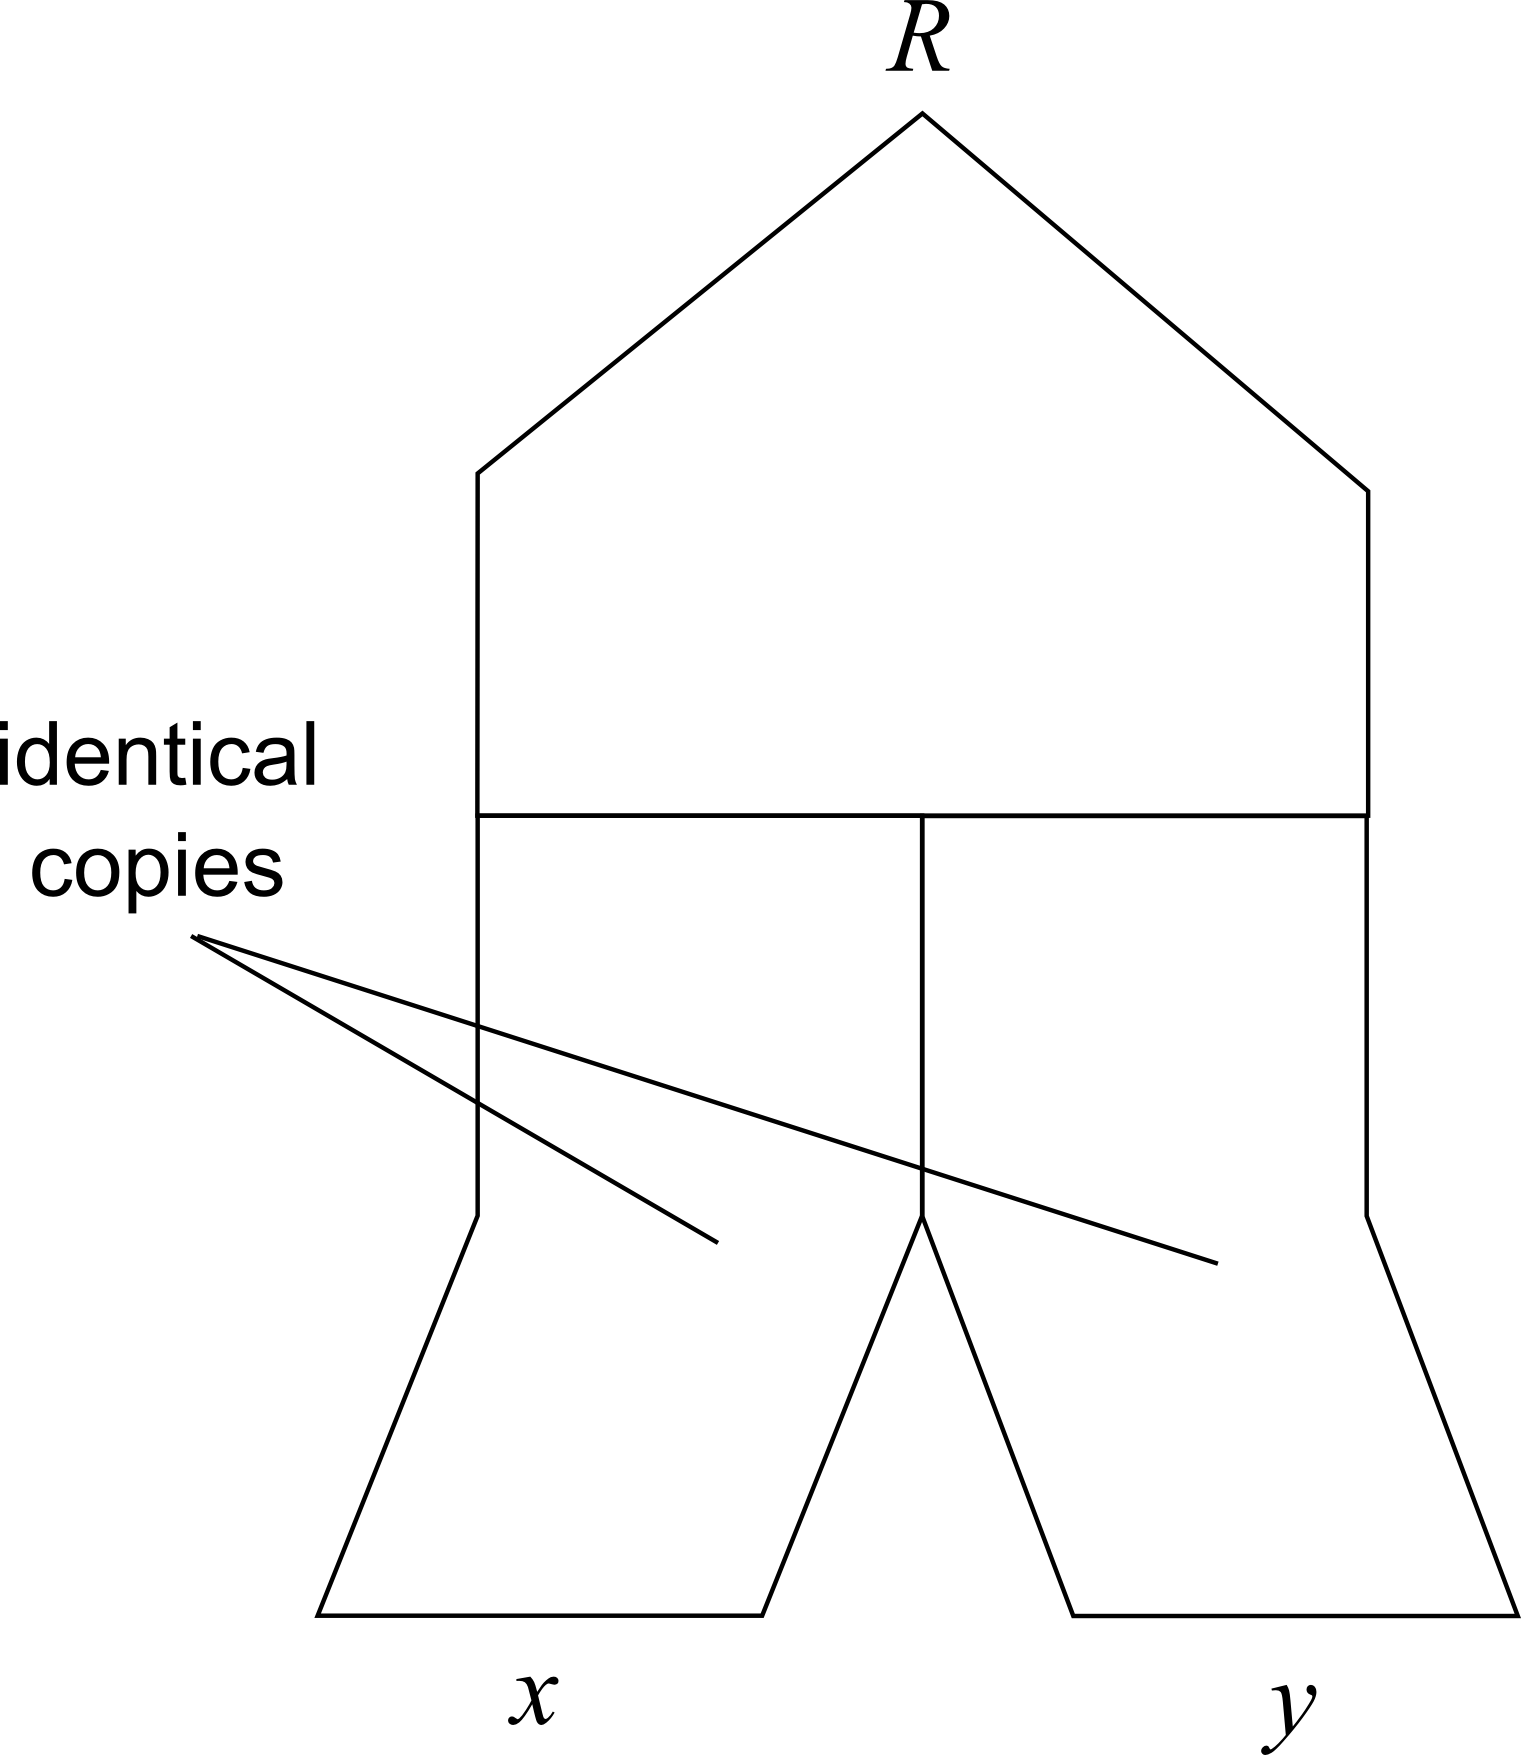
\includegraphics[scale=0.5]{R-network.png}
\end{equation}

或者,照旧是 feedforward network,但 somehow 它的学习是基於某 reward function。 问题是这 reward function 从何而来?  $R$ 可以是一个全部 $W$ 的函数,是由我们任意定义的。  

\clearpage
\section{Jacobian learning algorithm}

The classical Back Prop algorithm is \textbf{error-driven}, but in many AI problems the ``correct'' answers are not given, instead the feedback is provided via \textbf{rewards}. When an answer is correct, the reward $R > 0$, error $\mathscr{E} = 0$; when the answer is incorrect, $R < 0$, but $\mathscr{E}$ is still unknown (because we don't know the correct answer).  In other words, error-driven learning is inapplicable.

So I thought of a reward-driven learning method:  assume the neural network maps $\vect{x}_0 \mapsto \vect{y}_0$, usually it also maps the neighborhood of $\vect{x}_0$ to the neighborhood of $\vect{y}_0$.  If we wish to ``strengthen'' this pair of mapping, we can make a \textbf{bigger} neighborhood of $\vect{x}_0$ map to the same neighborhood close to $\vect{y}_0$.  We will make this precise.

This type of learning algorithm should be very useful to AI, and currently the author is not aware of other alternatives for training [deep] neural networks via rewards.

A feed-forward neural network can be constructed this way:
\begin{eqnarray}
\vect{y} &=& \vect{F}(\vect{x}) \\
\vect{y} &=& \sigmoid \stackrel{_L}{W} ... \sigmoid \stackrel{_\ell}{W} ... \sigmoid \stackrel{_1}{W} \vect{x}
\end{eqnarray}
where $W$ represents the matrix of \textbf{weights} on each layer $\ell$.

The \textbf{inverse} of $F$ is:
\begin{eqnarray}
\vect{x} &=& \vect{F}^{-1}(\vect{y}) \\
\vect{x} &=& \stackrel{_1}{\invW} \invsigmoid ... \stackrel{_\ell}{\invW} \invsigmoid ... \stackrel{_L}{\invW} \invsigmoid \; \vect{y}
\end{eqnarray}
Note: $\invW = W^{-1} \;,\; \invsigmoid = \sigmoid^{-1}$, the shape is different.

Assume that in the space of $\vect{x}$ there is a volume element $U$, which transforms via $\vect{F}$ to a volume element $V$ in the space of $\vect{y}$, then:
\begin{equation}
U = |J| \cdot V
\end{equation}
$\displaystyle J = \left[ \frac{\partial \vect{F}(x)}{\partial x} \right]$ is called the \textbf{Jacobian} matrix.

In our case, the value of $\displaystyle |J| = \left| \frac{\partial \vect{F}^{-1}(\vect{y})}{\partial \vect{y}} \right|$ at $\vect{y}_0$ represents ``the change in volume from $\vect{y}_0 \mapsto \vect{x}_0$''.  (Below, we will see that the direction of $\vect{F}$ or $\vect{F}^{-1}$ is not too important, as either way the computational complexity is essentially the same.)

Every time we get a \textbf{positive reward}, we can let the Jacobian $|J|$ increase slightly:
\begin{equation}
|J| := \det \left[ \frac{\partial \vect{F}^{-1}(\vect{y})}{\partial \vect{y}} \right]_{n \times n}
\end{equation}
The subscript indicates that it is a $n \times n$ matrix.

The meaning of the Jacobian matrix is:
\begin{equation}
J = \left[ \frac{\partial \mbox{ input}}{\partial \mbox{ output}} \right]
\end{equation}
The neural network's input and output are both of $\dim n$, so the Jacobian is naturally an $n \times n$ matrix.

To use \textbf{gradient descent}, we need to calculate these gradients: $\displaystyle \left[ \frac{\partial |J|}{\partial \vect{W}} \right]$, their total number is the number of weights in the network $= \sum \ell \; \#(\stackrel{_\ell}{W})$.

We need the formula for the derivative of the determinant:
\begin{eqnarray}
\frac{d}{dt} |A(t)| = tr ( \mbox{adj}(A) \cdot \frac{dA(t)}{dt} ) \\
\mbox{adj}(A) := |A| \cdot A^{-1}
\end{eqnarray}
In other words, for each weight $w := \stackrel{\ell}{W}_{ij}$, we need to calculate:
\begin{equation}
\frac{\partial}{\partial w} |J| = tr ( |J| \cdot J^{-1} \cdot \left[ \frac{\partial J}{\partial w} \right] )
\end{equation}
Note: $|J|$ and $J^{-1}$ are functions of $\vect{y}_0$, we only need to calculate them once outside the big loop.

Now a problem arises in the calculation of $\displaystyle \left[ \frac{\partial J}{\partial w} \right]_{n \times n}$:
\begin{equation}
\frac{\partial J}{\partial w} = \frac{\partial}{\partial w} \frac{\partial \vect{F}^{-1}}{\partial y} = \frac{\partial}{\partial w} \frac{\partial}{\partial \vect{y}} \; \stackrel{_1}{\invW} \invsigmoid ... \stackrel{_\ell}{\invW} \invsigmoid ... \stackrel{_L}{\invW} \invsigmoid \; \vect{y}
\end{equation}
This requires us to differentiation $W^{-1}$ w.r.t. $w$;  we can imagine the result would be very complicated.  So we use a trick, by ``reversing'' the network, we use $\invW$ to define the network weights, and then use $W = \invW^{-1}$ during forward propagation.

The components of $J$ are:
\begin{equation}
J_{ij} = \displaystyle \frac{\partial \vect{F}^{-1}_i}{\partial y_j} = \frac{\partial}{\partial y_j} \left[ \stackrel{_1}{\invW} \invsigmoid ... \stackrel{_\ell}{\invW} \invsigmoid ... \stackrel{_L}{\invW} \invsigmoid \; \vect{y} \right]_i =: \nabla^1_{i j} \\
\end{equation}
\begin{equation}
\begin{cases}
\nabla^1_{i j} &:= \displaystyle \sum_{k_1} [\, \stackrel{_1 \hspace{11pt}}{\invW_{i k_1}} \invsigmoid'(y^2_j) \nabla^2_{i j} \,] \\
\nabla^\ell_{i j} &:= \displaystyle \sum_{k_\ell} [\, \stackrel{_\ell \hspace{22pt}}{\invW_{k_{\ell - 1} k_\ell}} \invsigmoid'(y^{\ell + 1}_j) \nabla^{\ell + 1}_{i j} \,] \\
\nabla^L_{i j} &:= \quad \quad \displaystyle \stackrel{_L \hspace{21pt}}{\invW_{k_{L - 1} j}} \invsigmoid' (y_j)
\end{cases}
\end{equation}
This situation is exactly analogous to the classical Back Prop algorithm;  The above is just the application of the \textbf{chain rule}, with $\nabla^\ell$ written separately for each layer, therefore $\nabla$ is called the ``local gradient''.  The above formula amounts to propagating the entire network one time, where every weight appears \textbf{exactly once}.

But our work is not finished yet;  We need to calculate $\displaystyle \frac{\partial J_{ij}}{\partial \invw} =: \dot{\nabla}^1_{ij}$. \\
(Let's define $\invw := \stackrel{\ell}{\invW}_{g h} \;,\; k_0 := i \;,\; k_L := j$) \\
$\invw$ would be an element of $\invW$, but if $\invw \not\in \invW$, all the terms below would vanish:
\begin{equation}
\begin{cases}
\displaystyle \dot{\nabla}^1_{i j} = \sum_{k_1} \left[\, \stackrel{_1 \hspace{15pt}}{\invW_{i k_1}} \invsigmoid'(y^2_j) \dot{\nabla}^2_{i j}  \,\right] \\
\displaystyle \dot{\nabla}^\ell_{i j} = \sum_{k_\ell} \left[\, \stackrel{_\ell \hspace{15pt}}{\invW_{k_{\ell - 1} k_\ell}} \invsigmoid'(y^{\ell + 1}_j) \dot{\nabla}^{\ell + 1}_{i j} \,\right] \\
\displaystyle \dot{\nabla}^L_{i j} = \quad \quad \stackrel{_L \hspace{21pt}}{\invW_{k_{L - 1} j}} \invsigmoid' (y_j) \equiv 0
\end{cases}
\end{equation}
So what is left over is just this term:
\begin{eqnarray}
& \displaystyle \frac{\partial J_{ij}}{\partial \invw} = \sum_{k_1} \left[\, \stackrel{_1 \hspace{15pt}}{\invW_{k_0 k_1}} \invsigmoid'(y^2_j) ... \sum_{k_\ell} \left[\, \stackrel{_\ell \hspace{20pt}}{\invW_{k_{\ell - 1} k_\ell}} \invsigmoid'(y^{\ell + 1}_j) ... \right. \right. \\
& \begin{cases}
... \; \left. \left. \invsigmoid'(y^{\ell + 1}_j) \nabla^{\ell + 1}_{i j} \right] \right] \\
... \; \left. \left. \invsigmoid'(y^{\ell + 1}_j) \right] \right] \quad \quad \quad \mbox{if } \invw \in \mbox{last layer} \nonumber
\end{cases}
\end{eqnarray}
% \sum_{k_{\ell + 1}} (\, \stackrel{_{\ell + 1} \hspace{21pt}}{\invW_{k_\ell k_{\ell + 1}}} \invsigmoid' ... \; \stackrel{_L \hspace{21pt}}{\invW_{k_{L - 1} k_L}} \invsigmoid' (y_j) \;)) \\
% &:=& \sum_{k_1} (\, \stackrel{_1 \hspace{15pt}}{\invW_{k_0 k_1}} \invsigmoid'' ... \; \invsigmoid' (\vect{u}) \;)
The above formula means:  For each layer we repeat a block of $\left[ \sum \invW \; \invsigmoid \right]$, until we encounter $\invw = \stackrel{\ell}\invW_{g h}$, then we replace with the terminal form.

In contrast to classical Back Prop, the above formula gives us only one element in an $n \times n$ matrix;  From the complexity point of view, calculating the $\nabla$ for each weight is at least $n^2$ times as costly as classical Back Prop (even though we may re-use some intermediate computation results).  Recall that $n = \mbox{dim } \boxed{\mbox{state space}}$.

We can understand it thusly:  For each weight we try to calculate its influence towards the Jacobian, but the Jacobian is a \textbf{global} property of the network.  The key seems to lie in how each weight \textbf{influences} the Jacobian.

Now let's look back at this higher-level formula:
\begin{eqnarray}
\frac{\partial}{\partial w} |J| &=& tr ( |J| \cdot J^{-1} \cdot \left[ \frac{\partial J}{\partial w} \right] ) \\
&=& |J| \cdot tr ( \left[ \frac{\partial y}{\partial x} \right] \cdot \left[ \frac{\partial }{\partial w} \frac{\partial x}{\partial y} \right] ) \\
&=& |J| \cdot \sum_{i j} \left( \frac{\partial y}{\partial x} \right)_{i j} \left( \frac{\partial }{\partial w} \frac{\partial x}{\partial y} \right)_{i j}
\label{code-eqn2}
\end{eqnarray}

The most critical (slowest) part is the $(i, j) \in n \times n$ summation.  The first factor inside $\sum$ is the Jacobian $J$, the second factor is the $\nabla_w J^{-1}$ that we just calculated. 

% 比较一下经典 Back Prop 算法: 对每个 weight 我们会计算 ``local gradient'' $\displaystyle \nabla = \frac{\partial \mbox{ 误差}}{\partial w}$,但那个 $\nabla$ 比较易计算。

Back Prop's $\nabla$ has the form $\displaystyle \frac{\partial \, \boxed{\mbox{output}}}{\partial \, \boxed{\mbox{weights}}}$\\
whereas our $\nabla$ has the form $\displaystyle \left[ \frac{\partial}{\partial \, \boxed{\mbox{weights}}} \frac{\partial \, \boxed{\mbox{input}}}{\partial \, \boxed{\mbox{output}}} \right]_{n \times n}$.

In fact we just need to calculate the \textbf{approximate} direction and size of $\nabla_w |J|$.  Currently in our code we use this trick:  ignore the smaller terms in (\ref{code-eqn2}), so we don't need to do all of $n^2$ products. 

Or perhaps we can regard $|J|(\invw)$ as a function of the weight $\invw$, and then use its Taylor series expansion to approximate?

\bibliographystyle{plain} % or number or aaai ...
\bibliography{AGI-book}

\end{document}

\section{Misc logic....}

In LBAI the knowledge representation structure is built (\textit{fixed}) from the bottom up:
%\begin{equation}
%\mbox{words } \triangleright \mbox{ sentences } \triangleright \mbox{ logical form } \triangleright \mbox{ logical KB}
%\end{equation}
%Thus the structure of the KB is \textit{fixed} by the human designer. % This rigidity is perhaps why learning in logic-based systems is slow.

% In natural language, an idea can be expressed as a concatenation of words, for example:\\
% And it is just a short jump from word concatenations to symbolic logic.  But this jump may land us into a logic-based ``tar pit'', in which everything is theoretically possible, but often too slow in practice.

%It is just a short jump from the expression of ideas as word concatenations to logical form as linear (or tree-like, or graph-like) compositions of symbols:
\begin{equation}
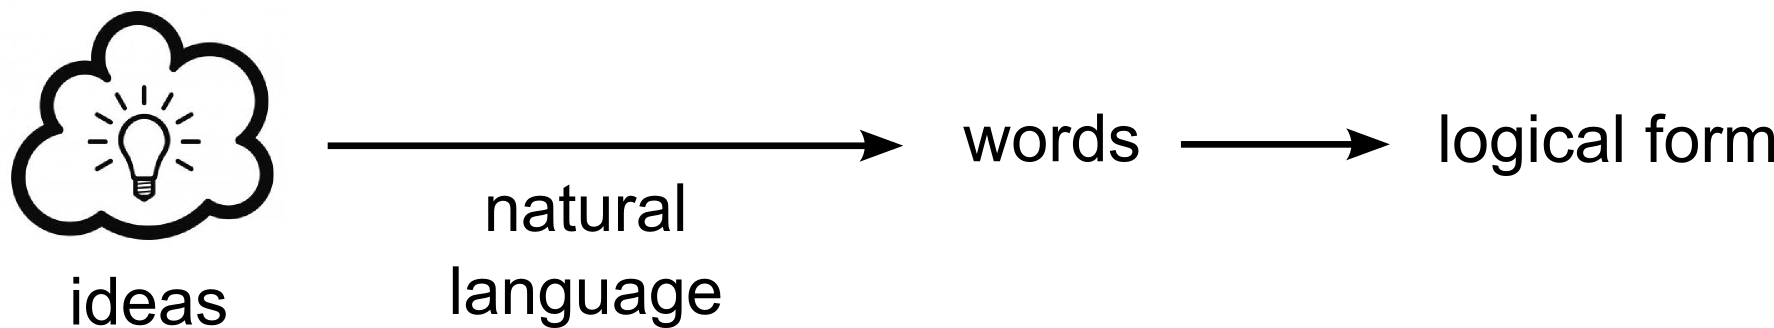
\includegraphics[scale=0.5]{ideas-vs-logical-form.png}
\end{equation}
but is it valid (or profitable) to assume that our mental representations are \textit{isomorphic} to such logical structures?  Or drastically different?

Humans are good at designing symbolic structures, but we don't know how to design \textit{neural} representations which are more or less opaque to us.
Perhaps we could use a neural network acting recurrently on the state vector to \emp{induce} an internal representation of mental space.  ``\textit{Induced by what},'' you ask?  By the very structure of the neural network itself.  In other words, forcing a neural network to \textit{approximate} the ideal operator $R^*$.

From an abstract point of view, we require:
\begin{itemize}
\item $R$ be an endomorphism: $X \rightarrow X$
\item $R$ has a learning algorithm: $R \stackrel{A}{\longmapsto} R^*$
\end{itemize}

$R$ would contain all the knowledge of the KB, so we expect it to be ``large'' (eg. having a huge number of parameters).  We also desire $R$ to possess a \emp{hierarchical} structure because hierarchies are computationally very efficient.  A multi-layer perceptron (MLP) seems to be a good candidate, as it is just a bunch of numbers (weight matrices $W$) interleaved by non-linear activation functions:
\begin{equation}
R(\vect{x}) = \sigmoid(W_1 \sigmoid(W_2 ... \sigmoid(W_L \vect{x} )))
\end{equation}
where $L$ is the number of layers.  MLPs would be our starting point to explore more design options.

In 1991 Siegelmann and Sontag \cite{Siegelmann1991} proved that recurrent neural networks (RNNs) can emulate any Turing machine.  In 1993 James Lo \cite{Lo1993} proved that RNNs can universally approximate any non-linear dynamical system.

The idea of $R$ as an operator acting on the state is inspired by the ``consequence operator'' in logic, usually denoted as $\mbox{Cn}$:
\begin{equation}
\mbox{Cn}(\Gamma) = \{ \mbox{ set of propositions that entails from } \Gamma \; \}
\end{equation}
but the function of $R$ can be broader than logical entailment.  We could use $R$ to perform the following functions which are central to LBAI:
\begin{itemize}
\item \emp{deduction} -- forward- and backward-chaining
\item \emp{abduction} -- finding explanations
\item \emp{inductive learning}
\end{itemize}

\begin{tcolorbox}[width=\textwidth,colback={white},title={\centering \emp{Example 1: } primary-school arithmetic},colbacktitle=white,coltitle=black]

A recurrent neural network is a \textit{much more powerful} learning machine than a feed-forward network, even if they look the same superficially.

\begin{wrapfigure}{l}{2cm}
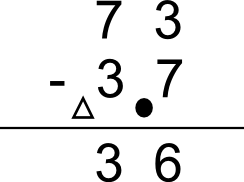
\includegraphics[scale=0.6]{elementary-arithmetic.png}
\end{wrapfigure} 

As an example, consider the way we perform 2-digit subtraction in primary school.  This is done in two steps, and we put a dot on paper to mark ``carry-over''.

The use of the paper is analogous to the ``tape'' in a Turing machine -- the ability to use short-term memory allows us to perform much more complex mental tasks.

We did a simple experiment to train a neural network to perform primary-school subtraction.  The operator is learned easily if we train the two steps \textit{separately}.  The challenge is to find an algorithm that can learn \emp{multi-step} operations by itself.

\end{tcolorbox}

\begin{tcolorbox}[width=\textwidth,colback={white},title={\centering \emp{Example 2: } variable binding in predicate logic},colbacktitle=white,coltitle=black]

The following formula in predicate logic defines the ``grandfather'' relation:

\begin{equation}
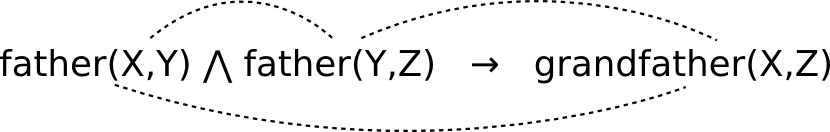
\includegraphics[scale=0.75]{linkage-in-logic-variables.png}
\end{equation}


We did a simple experiment to train a neural network to perform primary-school subtraction.  The operator is learned easily if we train the two steps \textit{separately}.  The challenge is to find an algorithm that can learn \emp{multi-step} operations by itself.

\end{tcolorbox}  

In LBAI, logic possesses additional structure:
\begin{itemize}
\item \emp{truth values} (eg. P(rain tomorrow) = 0.7)
\item \emp{propositional structure} (eg. conjunction: $A \wedge B$) 
\item \emp{sub-propositional structure} (eg. predication: loves(john, mary) )
\item \emp{subsumption structure} (eg. $\mbox{dog} \subseteq \mbox{animal}$)
\end{itemize}

These structures can be ``transplanted'' to the vector space $X$ via:
\begin{itemize}
\item \emp{truth values: } an extra dimension conveying the ``strength'' of states
\item \emp{propositional structure: } eg. conjunction as vector addition,
\begin{equation}
A \wedge B = \vect{x}_A + \vect{x}_B + ...
\end{equation}
but we have to avoid linear dependencies (``clashing'') such as:
\begin{equation}
\vect{x}_3 = a_1 \vect{x}_1 + a_2 \vect{x}_2
\end{equation}
This would force the vector space dimension to become very high.
\item \emp{sub-propositional structure: } eg. tensor products as composition of concept atoms:
\begin{equation}
\mbox{loves(john, pete)} = \overrightarrow{john} \otimes \overrightarrow{love} \otimes \overrightarrow{pete}
\end{equation}
\item \emp{subsumption structure: } eg. define the positive cone $C$ such that
\begin{equation}
\mbox{animal} \supseteq \mbox{dog} \quad \Leftrightarrow \quad \overrightarrow{animal} - \overrightarrow{dog} \in C
\end{equation}
\end{itemize}

But the more logical structure we add to $X$, the more it will resemble logic, and this whole exercise becomes pointless.  Remember our original goal is to try something different from logic, by \textit{relaxing} what defines a logical structure.  So we would selectively add features to $X$.


\section{Unifying RL and RNN}

From the viewpoint of reinforcement learning, we aim to learn the \emp{policy} function: \par
\begin{equation}
\begin{tikzcd}[]
\mbox{policy : ~~state} \arrow[r, mapsto, "\scalebox{0.8}{action}"] & \mbox{state'}
\end{tikzcd}
\end{equation}
Where $K$ can be regarded as the \emp{mental state}, and thus an \emp{action} in RL turns $K$ into $K'$.

In our system, there are 2 pathways that act on $K$, via RNN and RL respectively: \par
\begin{equation}
\begin{tikzcd}[column sep=huge]
& K'_1 \arrow[dd, dashed, no head, "\scalebox{1.3}{$\approx$}"] \\
K \arrow[ur, "\mbox{RL}"] \arrow[dr, "\mbox{RNN}"'] & \\
& K'_2
\end{tikzcd}
\end{equation}
In RL, the action $a$ acts on $K$, whereas in RNN, $R$ acts on $K$.

\emp{Note}: RNN and RL are learning algorithms, and if they are both applied to the same problem, conflicts will necessarily arise, unless there is a way to combine them.

At state $K$, we estimate the Q-value $Q(K \stackrel{a}{\mapsto} K')$.  The action that would be chosen at state $K$ is $\displaystyle \arg\max_a Q(K \stackrel{a}{\mapsto} K')$.  This could be used to train the RNN via $\displaystyle K \vdash_W ...^n K'$.

RL 在众多状态 $K$ 之间游荡,学习 $Q(K \mapsto K')$。  因为 RL 独有奖励讯息,我们必需用 RL 来教导 RNN 学习,反之不可。  第一个问题是: RL 如何在 $K$ 之间游荡?   游荡是随机的,但也可以借助 RNN 的随机性、或在 RNN 自身的游荡中注入更多随机性、或者根本就是 RL 自己产生的随机性。  接下来的问题是: RNN 如何用 $Q$ 值来诱发学习?

RNN 的 ``$n$-fold'' 学习可以通过以下方式实现: 
\begin{itemize}
\item stochastic forward-backward propagation
\item genetic?
\item 最有趣的是 Hebbian learning,因为它似乎特别适合这情况。  
\end{itemize}

RNN 的本质是什么?  它似乎是一个 recurrent hetero-associative memory。  但其实它还需要将 input 作类似於 Word2vec 的 encoding。  这个 encoding 将「相似」的思维状态 $K$ 归到同类。  利用空间中的相似度,RL 可以用一些连续函数来近似 Q 值(详细情况还有待分析)。

另一个问题是: 虽然用函数的近似可以做到 generalization,但另一个方法是利用状态 $K$ 中的空位作暂时储存。 这两者似乎很不同。  问题似乎在於: 状态转换 $K \mapsto K'$ 是不是对应於逻辑中的\emp{一条} rule?  答案似乎是 yes。  这个共识是很重要的。  如果用 decision tree,需要的是向量空间中的相似度。

现在的关键是「状态变量」。  因为它可以做到符号逻辑中靠变量的 generalization,这是前所未有的。  这种 generalization 似乎不需要相似度,因为它是符号的!  会不会在向量空间中的状态变量 能够做到之前逻辑变量做不到的动作?  不管怎样,用 RNN 学习这些变量的动作似乎是很难的,因为这些动作似乎不是对\emp{误差}的梯度下降。  除非这些动作本身也近似於其他动作,但那是怎样的近似?  学习 multi-step logic 其实和以前的 forward / backward chaining 没有分别!  唯一分别是命题的 representation 改变了,它未必像符号的 concatenation。  所以问题仍然是 ``$n$-fold'' 学习法。 

而且注意: RL 的 generalization 根本上不同於 rules 空间中的 generalization。 前者是思维空间 $K$ 中的一般化,后者也可以是 $K$ 空间的一般化,但也可以是依赖「状态变量」的一般化。

一般来说,RL 和 RNN 的行动和学习,是可以互相独立的。  

还有 heterarchical 的分类法。  想用 decision tree 或什么,达到不同网络的\emp{分工}。  在组织知识这方面,深度网络有没有用?  可以想像,在视觉识别中,在网络的最上层有很多 objects,而它们都可以还原到底层的 features。  网络有更多层,可以识别的事物更抽象。  但现在我们要的不是\emp{模式识别},而是 mapping。 特别是抽象模式的 mapping。  想要的是: 大量的 rules,将不同的 $K$ 映射到新的 $K'$。

还有一点要澄清的是: 究竟每一个「思元素」在向量空间中是不是\emp{一点}?  如果有了这个「思元素 = 点」假设,则每次 iteration 应该会删除一个思元素,而用另一个(全新的)思元素取代之。  这样,$K \mapsto K'$ mapping 就有了更确定的结构。  这样的 setup 已经很接近 logic 系统,但其学习算法仍然很有 combinatorial 的 ``feel''。 (因为只有当两个 rules 串连之后,才能达到某个结论,而这个串连有没有中间的 continuous 状态?)  这种串连通常是怎样找到的?  

现在有一转机: 如果「思元素 = 点」,则「状态变量」的形成似乎会很普遍,而我们可以集中研究如何学习 single-step rules。 RL 的 rewards 可以指导学习,但这些「终极 rewards」对学习的细节没有指导作用。  我们似乎可以用「\emp{时间延迟}」来达到「状态变量」的效果,这个做法无形中增加了使用状态变量的机会。  

现在总结一下仍然有待回答的问题:
\begin{itemize}
\item RL 的 generalization 如何做?
\item iterative thinking map 如何 learn?
\item 
\end{itemize}

Hebbian 的情况是: 有某一 I/O pattern; 我想 strengthen 这 pattern。 

Assuming the learning is correct, $K'_1$ and $K'_2$ should be roughly the same \textemdash~ but this ignored the possibility that one path may take multiple steps to converge with the other path.  \footnote{This situation has been encountered in term rewriting systems (TRS):  If in a TRS any 2 different rewriting paths always converge to the same result, it is said to have the \emp{Church-Rosser property}.  For example the $\lambda$-calculus invented by Church has this property.} 

Now I stipulate that $R$ be more ``refined'', that is to say, applying $D^n$ times may be equivalent to applying $a$ once:
\begin{equation}
\begin{tikzcd}[column sep=huge]
& K'_1 \arrow[dd, dashed, no head, "\scalebox{1.3}{$\approx$}"] \\
K \arrow[ur, "\scalebox{1.3}{$a$}"] \arrow[dr, "{\scalebox{1.3}{$D^n$}}"'] & \\
& K'_2
\end{tikzcd}
\end{equation}
Using a different notation, $a$ is the \emp{restriction} or \emp{section} of $D^n$ at point $K$: $a = D^n|_K$.

Now the question is, do the RNN and RL paths have any \textit{essential} difference?
\begin{itemize}
\item Their internal \emp{representations} are different:\par
\dashh RNN is a multi-layer neural network\par
\dashh RL's representation is $Q(\mbox{state},\mbox{action})$, usually stored as a \textit{look-up table}, although $Q$ could be approximated by a neural network as well.
\item RL learns through \emp{rewards}, RNN learns from \emp{errors}.  Thus RL has broader applicability, because not all questions have ``correct answers'' that could be measured by errors.  In RL we just need to praise Genifer whenever she displays good behavior.
\item The internal cognitive state $K$ exists because of RNN:  it is simply the vector input and output of the RNN.  Without this $K$, RL would be clueless as to what are its internal states.  It can be said that the RNN provides a \textit{machinery} for RL to control.
\end{itemize}

% programming needed:
% RNN: with special back-prop
% RL: approximate Q(K,a), using special NN that can find max also

% 整体来说,RL 可以操控的 actions 包括:
% \begin{enumerate}[\tab (A)]
% \item apply $K \stackrel{D}{\mapsto} K'$ \par
% 但注意: $K$ 是认知状态,$R$ 是对 $K$ 进行「合乎逻辑的推论」。 所以,无论发生什么事,我们都会将 $R$ 作用在 $K$ 上几次。 换句话说,$R$ 是\ds{必然}进行的动作,或者可以看成是在\ds{背景}下进行的运作,所以不需要用 RL 学习。 %RL 的用处是学习如何在很多 actions 之间选择最好的一个,所以 $R$ 不是 RL 需要学习的 action,它只是。

% \item 改写认知状态 $K \mapsto K'$ \par
% RL 的 actions (A) 是
% 在思考过程中改变 $K$ 的值。 例如我们得到一个局部结论,这个局部结论的状态不是最终答案,但也比什么都没有的效用更高。 改写 $K$ 的方法可以是: 例如 将 $K \mbox{ += } \delta K$,或者 「if $K \in$ 某 region,then $K \mbox{ += } \delta K $」。

% \item 学习: change $R$ \par

From the perspective of reinforcement learning, we could reward some results of multi-step inference: \par
\begin{equation}
\begin{tikzcd}[row sep=tiny]
x_0 \arrow[r, mapsto, "a"] & x_\vdash \quad \updownarrow \bigstar
\end{tikzcd}
\end{equation}
$\updownarrow \bigstar$ means ``to give positive or negative rewards''.  We want to learn $a$ which is the action to be taken at state $K$.  The learning algorithm is based on the famous \emp{Bellman optimality condition} (see next section).

Perhaps we should use RL to \textit{guide} the learning in RNN, as RNN is more fine-grained....

To combine the 2 learning approaches, we could use the technique of \emp{interleaving}: for each step apply RL once, apply RNN $n$ times.

% 但 $R$ 本身是 RNN,它还可以透过 back-prop 进行学习,两者似乎是不同的。  Back-prop 是透过 $\frac{\partial}{\partial D}(\mbox{error})$ 的梯度来学习。

The learning in RNN may also involve \emp{neurogenesis} (adding new neurons and connections), but I have not considered this aspect yet.

% RNN 的 $R$ 也是将 $K$ 变成 $K'$ 的作用:\par
%\begin{figure}[h]
%\centering
%\begin{tikzcd}[row sep=tiny]
%K \arrow[r, mapsto, "\scalebox{1.3}{$R$}"] & K'
%\end{tikzcd}
%\end{figure}
% $R$ 和 RL 的 actions 是不一样的。

There are 4 learning modes:
\begin{itemize}
\item learning to listen/talk
\item RL-based learning
\item inductive learning
\end{itemize}

\section{Misc points}

\begin{itemize}
\item If sigmoid is replaced by polynomial, universal approximating property may be retained.

\item Banach fixed point theorem does not apply because $R$ in general need not be contractive.  Question is whether $R$ necessarily converges to fixed points and the answer is no.

\item If reasoning operator $R$ is continuous, the flow of the dynamical system is governed by an autonomous differential equation.  Poincare-Bendixson only applies to dynamical systems on the plane, and is irrelevant to systems whose phase space has dimension $\geq 3$, or to discrete dynamical systems.

\item Time can be discrete or continuous.

\item Goal is to find minimizer of error (ie, to approximate a function given some input-output data points).  The (finite) set of local minima can be solved via setting $\frac{\partial R}{\partial W} = 0$.  The number of local minima can be calculated as: ?  McClelland paper.

\item If operator is discontinuous, what advantages can be gained?
\end{itemize}

What I want to do now is to determine if $R$ implemented as a deep network is sufficient to model human-level reasoning.

One principle seems to be that logical conclusions must not proliferate indefinitely.  But we are not sure what kind of structural constraints this would impose on the vector space.  Or whether we should impose such constraints manually.

What other properties are desired for the implementation of $R$?

\section{Architecture}

First, cartoon version:
\begin{equation}
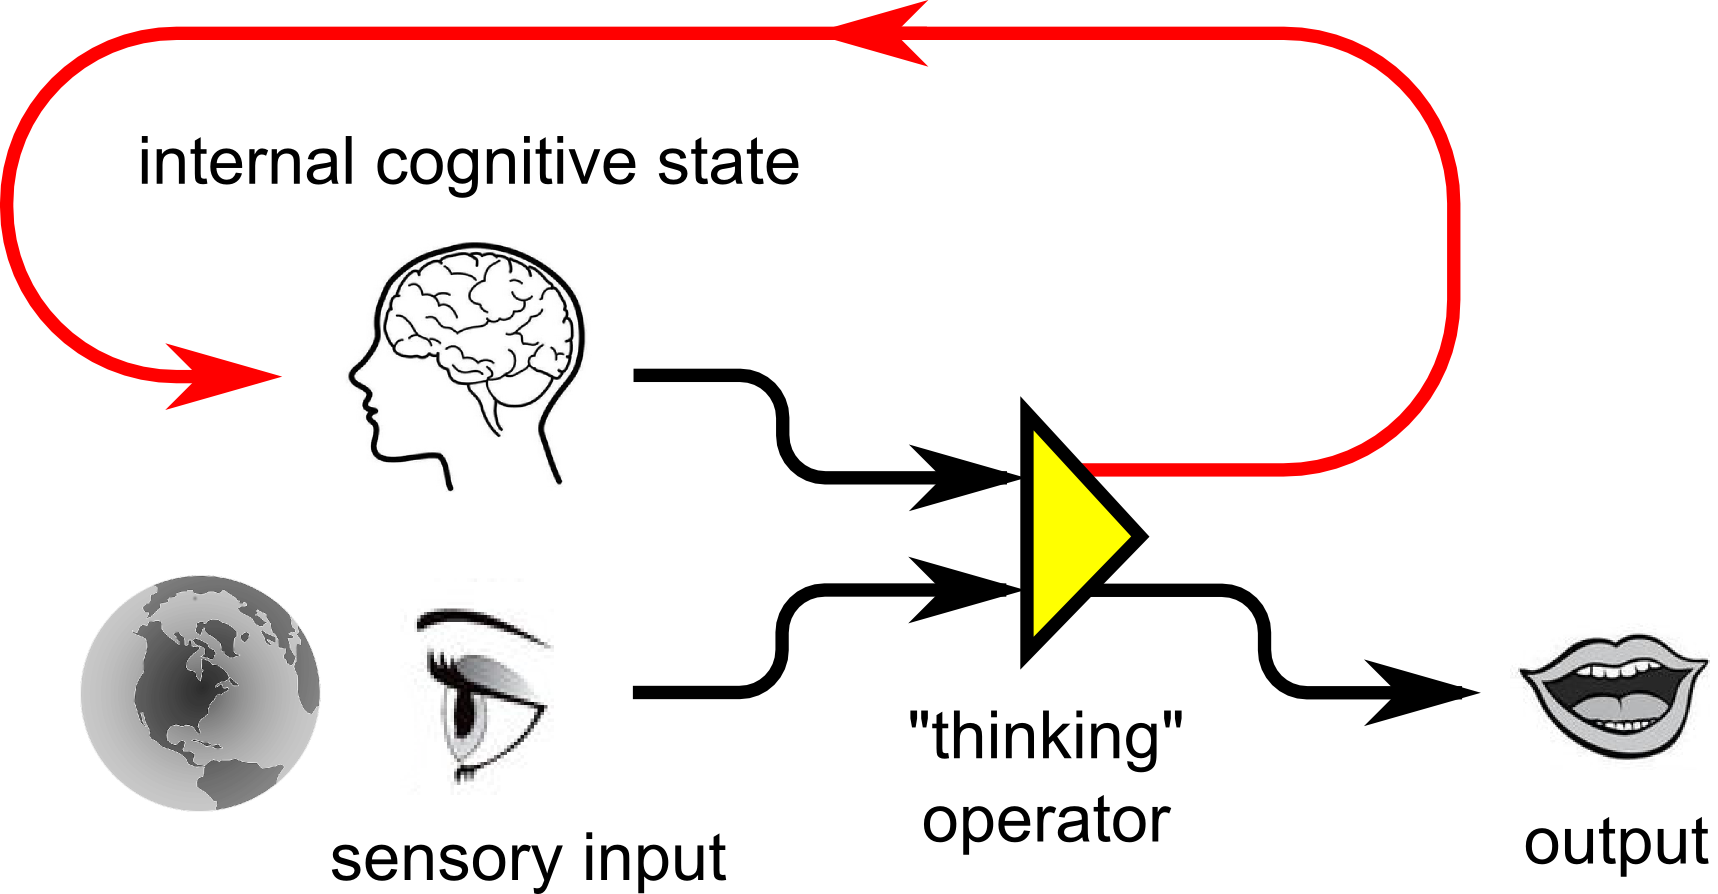
\includegraphics[scale=0.5]{architecture-cartoon.png}
\end{equation}

\begin{equation}
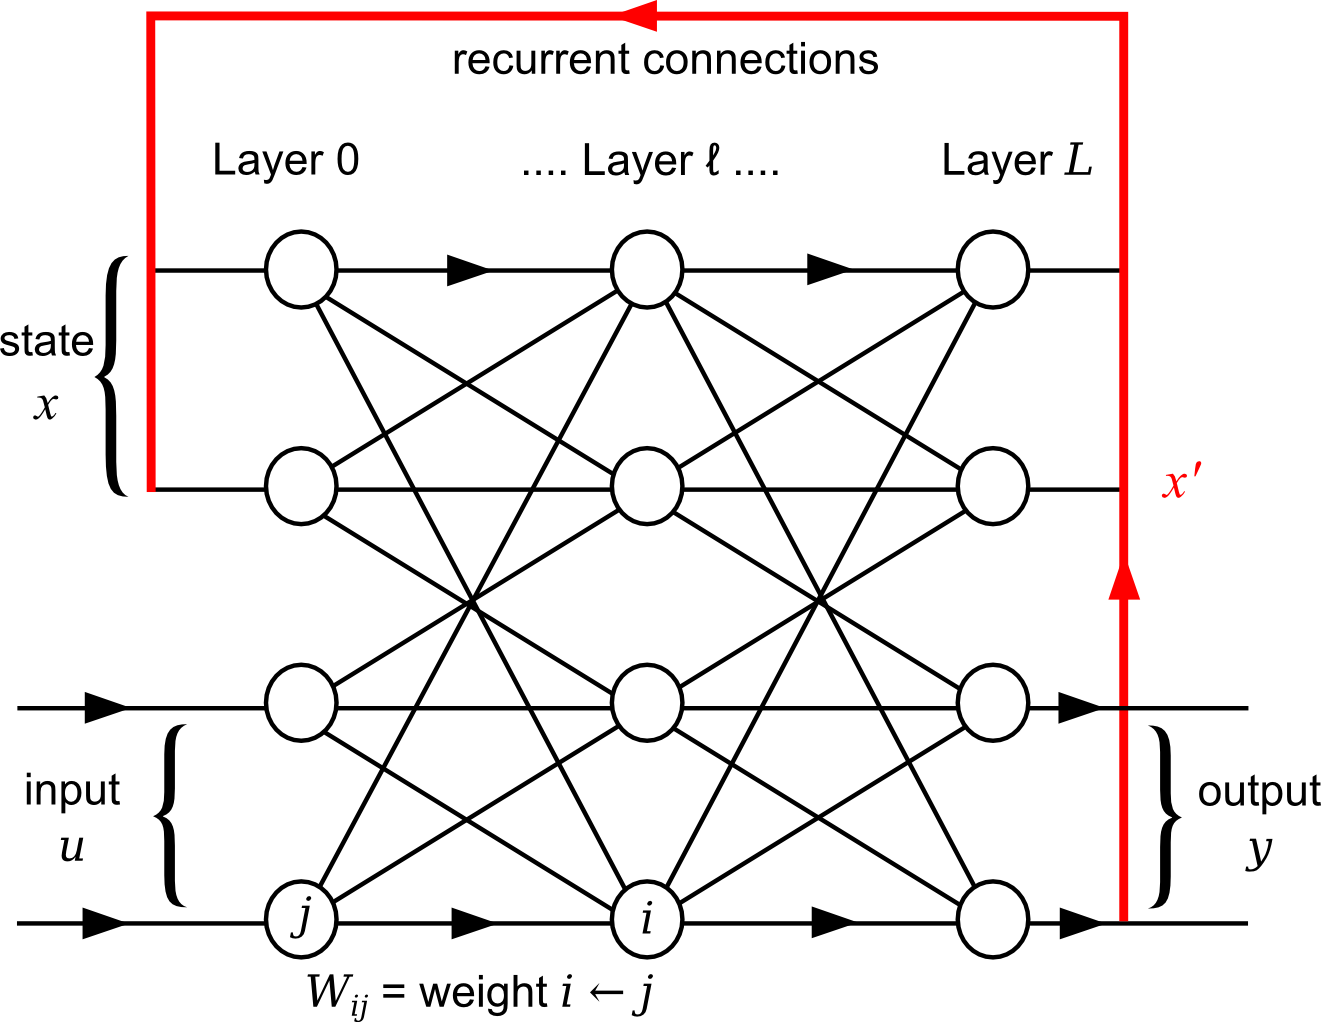
\includegraphics[scale=0.5]{RNN-topology.png}
\end{equation}

TO-DO:  The state space $X$ may be too large and we may need an \emp{attention mechanism} to select some parts of $X$ for processing by $R$.  This is the notion of \emp{working memory} in cognitive science.
\begin{equation}
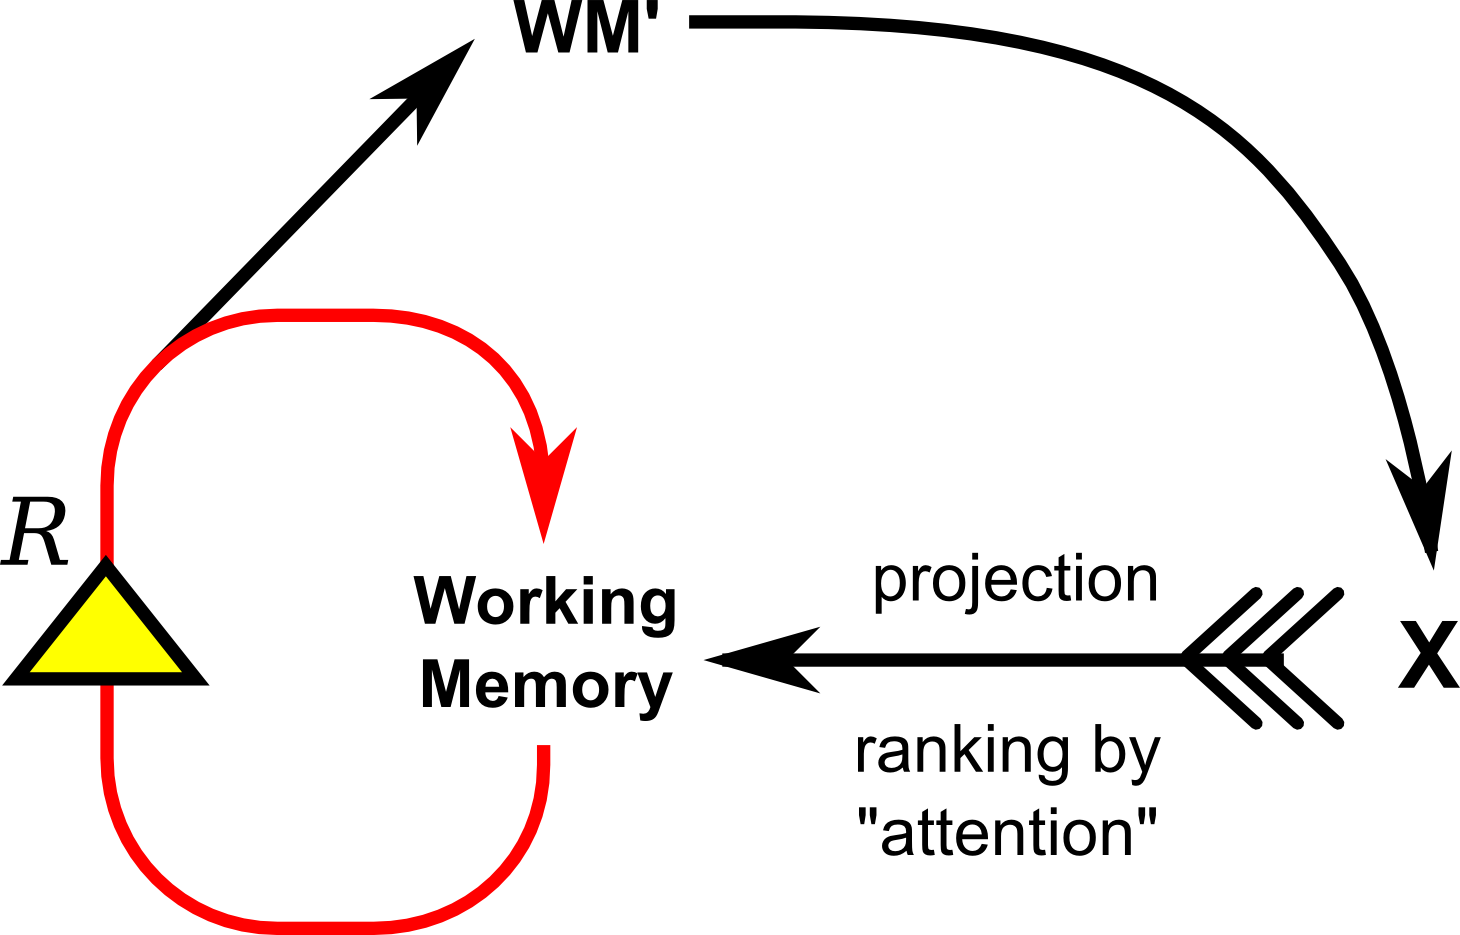
\includegraphics[scale=0.4]{working-memory.png}
\end{equation}

\section{Deep Recurrent Learning}

The learning algorithm for $R$ is central to our system.  $R$ learns to recognize input-output pairs $( \vect{x}_0, \vect{x}^* )$.  What makes it special is that $R$ is allowed to iterate a \textit{flexible} number of times before outputting an answer.  In feed-forward learning we simply learn single-pass recognition, whereas in common recurrent learning we train against a \textit{fixed} time sequence.  Here, the time delay between input and output is allowed to stretch arbitrarily.

Suppose the recurrent network $R$ iterates $n$ times:
\begin{equation}
\vect{x}_{t+1} = \overbrace{R \circ R \circ ...}^{n} (\vect{x})
\end{equation}

As $n \rightarrow \infty$, we get the continuous-time version (a differential equation):
\begin{equation}
\frac{d\vect{x}(t)}{dt} = \mathfrak{R}(\vect{x}(t))
\end{equation}

We could run the network $R$ for a long enough time $T$ such that it is highly likely to reach an equilibrium point.  Then:
\begin{equation}
\vect{x}_{T} = \int_0^T \mathfrak{R}(\vect{x}(t)) dt
\end{equation}
and the error:
\begin{equation}
% \mathscr{E} = \vect{x}^* - \vect{x}_{T}
\boxed{误差} = \vect{x}^* - \vect{x}_{T}
\end{equation}
where $\vect{x}^*$ is the target value which is independent of time.
\begin{eqnarray}
\frac{\partial\mathscr{E}}{\partial\vect{W}} &=& - \frac{\partial}{\partial\vect{W}} \int_0^T \mathfrak{R}(\vect{x}(t)) dt \nonumber \\
&=& - \frac{\partial}{\partial\vect{W}} \int_0^T \sigmoid(W_1 \sigmoid(W_2 ... \sigmoid(W_L \vect{x}(t))) dt
\end{eqnarray}

When there are many layers or if the recurrence is too long, back-prop learning becomes ineffective due to the \emp{vanishing gradient} problem.  One solution is to use the \emp{rectifier} activation function:
\begin{equation}
\rectifier (x) = 
\begin{cases}
x, & \mbox{if } x \geq 0 \\
0, & \mbox{otherwise}
\end{cases}
\end{equation}
Since its derivative is piecewise constant, it does not suffer from the vanishing gradient problem.

\subsection{Forward-backward Algorithm}

This is inspired by forward- and backward-chaining in LBAI.  We propagate the state vector from both the initial state $\vect{x}_0$ as well as the final state $\vect{x}^*$.  This bi-directional propagation is added with noise and repeated many times, thus implementing a \emp{stochastic local search}:

\begin{equation}
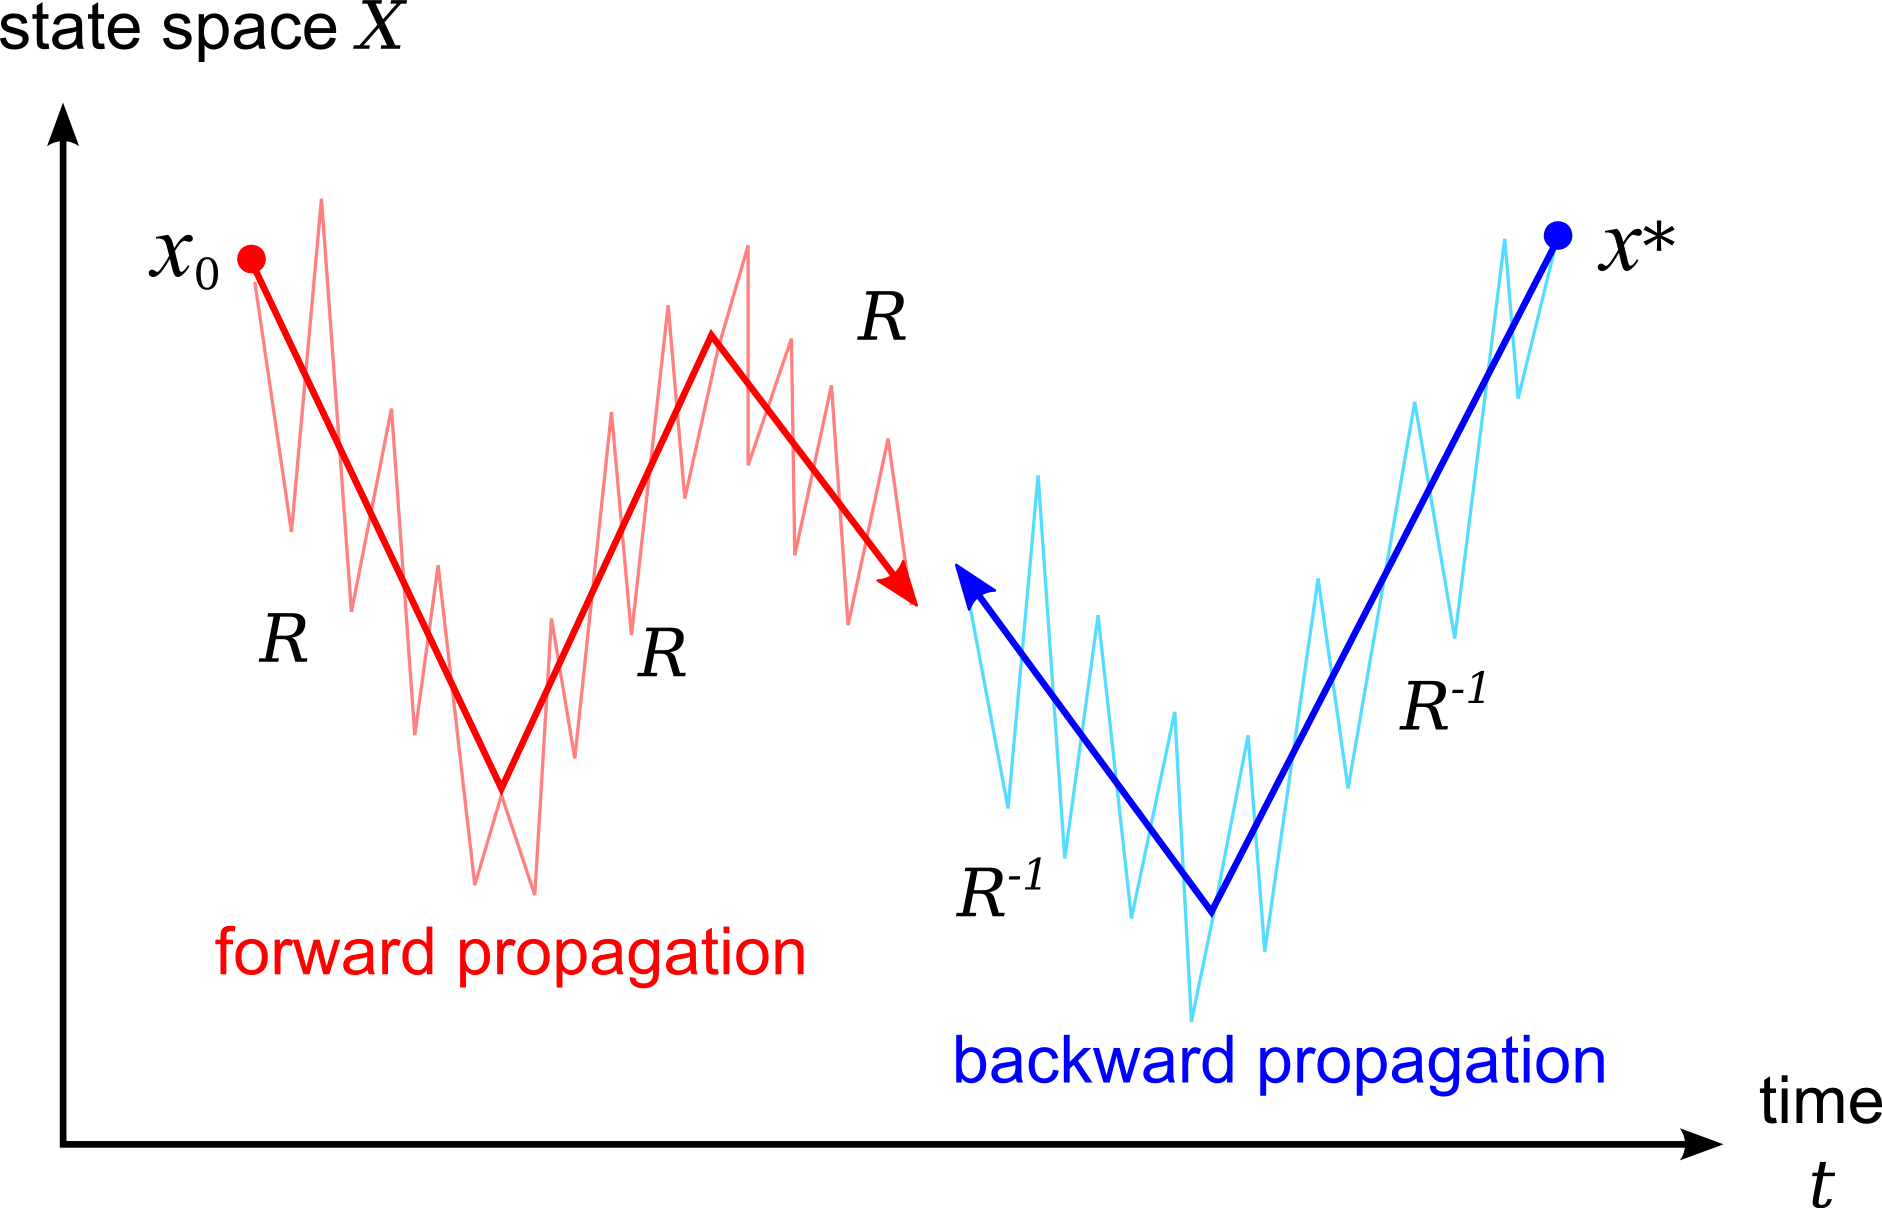
\includegraphics[scale=0.6]{forward-backward-algorithm.png}
\end{equation}

When the forward and backward states get close enough, a successful path is found, and we record the gap and the noises along the path, and use them to train $R$ so that this new path would be recognized.

% One key question is how to deal with "don't care" bits?  One answer is that their errors are zero.  But then this is the same as the error for "correct" weights, which seems not well.  There's got to be a way to alter weights when the answer is correct...

% For \# Iteration = 0, output is immediately known, so potentially the training can be done.  But how to convey that all these alterations of weights are \emp{optional}?

\section*{Acknowledgements}

\footnotesize{In a forum discussion with Ben Goertzel dated 25 June 2014 on the AGI mailing-list: (artificial-general-intelligence @googlegroups.com), YKY asked: Why bother with neural networks, which typically require many neurons to encode data, when logic-based AI can represent a proposition with just a few symbols?  Ben's insight is that neural networks are capable of learning its own representations, and their learning algorithms are relatively fast.  We have been working on "neo-classical" logic-based AI for a long time, and begin to realize that inductive learning in logic (based on combinatorial search in a symbolic space) is perhaps \textit{the bottleneck} in the entire logic-based paradigm.  So we try to look for alternatives that might enable learning to be faster, though we would still emphasize that logic-based AI remains a viable approach to AGI. %, provided that the right search heuristics be found (most probably in the form of \emp{hierarchical organization} of the learning space).
}

\bibliographystyle{plain} % or number or aaai ...
\bibliography{AGI-book}

\end{document}
